\documentclass{article}
\usepackage{iclr2026_conference,times}
\usepackage{booktabs}
\usepackage{array}
\usepackage{amsmath}
\usepackage{amssymb}
\usepackage{graphicx}
\usepackage{multirow}
\usepackage{hyperref}
\hypersetup{hidelinks}
\usepackage{url}
\usepackage{needspace}
\usepackage{enumitem}
\usepackage{placeins}
\usepackage{float}
\usepackage{longtable}

% Keep appendix-only float pages top-aligned instead of vertically centering a
% single data table in a large blank field.
\makeatletter
\setlength{\@fptop}{0pt}
\makeatother

% R48 layout fix: permit ragged page bottoms so a pushed large appendix [H]
% table leaves ordinary bottom whitespace instead of an overfull \vbox.
\raggedbottom
\widowpenalty=10000
\clubpenalty=10000
\displaywidowpenalty=10000



\usepackage{xcolor}
\setlength{\parskip}{2pt plus 0.5pt minus 0.5pt}

\title{Null Calibration for Multiple-Choice Evaluation: When ``Above Chance'' Fails the Input-Blind Floor}
\author{Anonymous authors \\ Paper under double-blind review}

\begin{document}

\maketitle

\begin{abstract}
Multiple-choice scores are commonly interpreted relative to nominal chance, even when an input-blind predictor can do better. We separate two reporting questions. For interface comparison, an arm-independent reference uses the construct's best constant input-blind predictor. For item-level information in one arm, an arm-conditional permutation null preserves the arm's prediction marginal within option-count strata. The first reference is a one-directional reporting check, not a certificate of construct validity; the second assigns every pure constant emitter exactly zero regardless of its collapse letter.

The best-constant floor must itself be calibrated under a null that the construct can realise. Restricting that null to each item's legal letters leaves only MMLU and BoolQ with label floors that a balanced null could not plausibly produce; for the other letter constructs, the analysis motivates a different reference without establishing a floor--chance difference in magnitude. On MMLU-Pro, only 1/12 non-OLMo cells clears the best-constant floor under the matched paired-bootstrap standard. Across five smaller benchmarks, 9/85 designated damaged cells clear the floor on the interval standard, all of them healed OLMo-2 arms; achieved precision explains why most per-benchmark tests remain inconclusive (Table~\ref{tab:headline-reference}).

Applying the arm-conditional null to 27 cells withdraws one above-floor capability label, removes both below-floor competence labels, and exposes a weak intact-family anchor. Full-fp32 evaluation eliminates every bf16 exact tie without recovering accuracy, so exact numerical ties do not explain the observed failure. These results support a practical rule: state the construct-specific input-blind reference, its uncertainty, and its intended inferential role before interpreting arm differences.
\end{abstract}

\begin{figure}[!htbp]
    \centering
    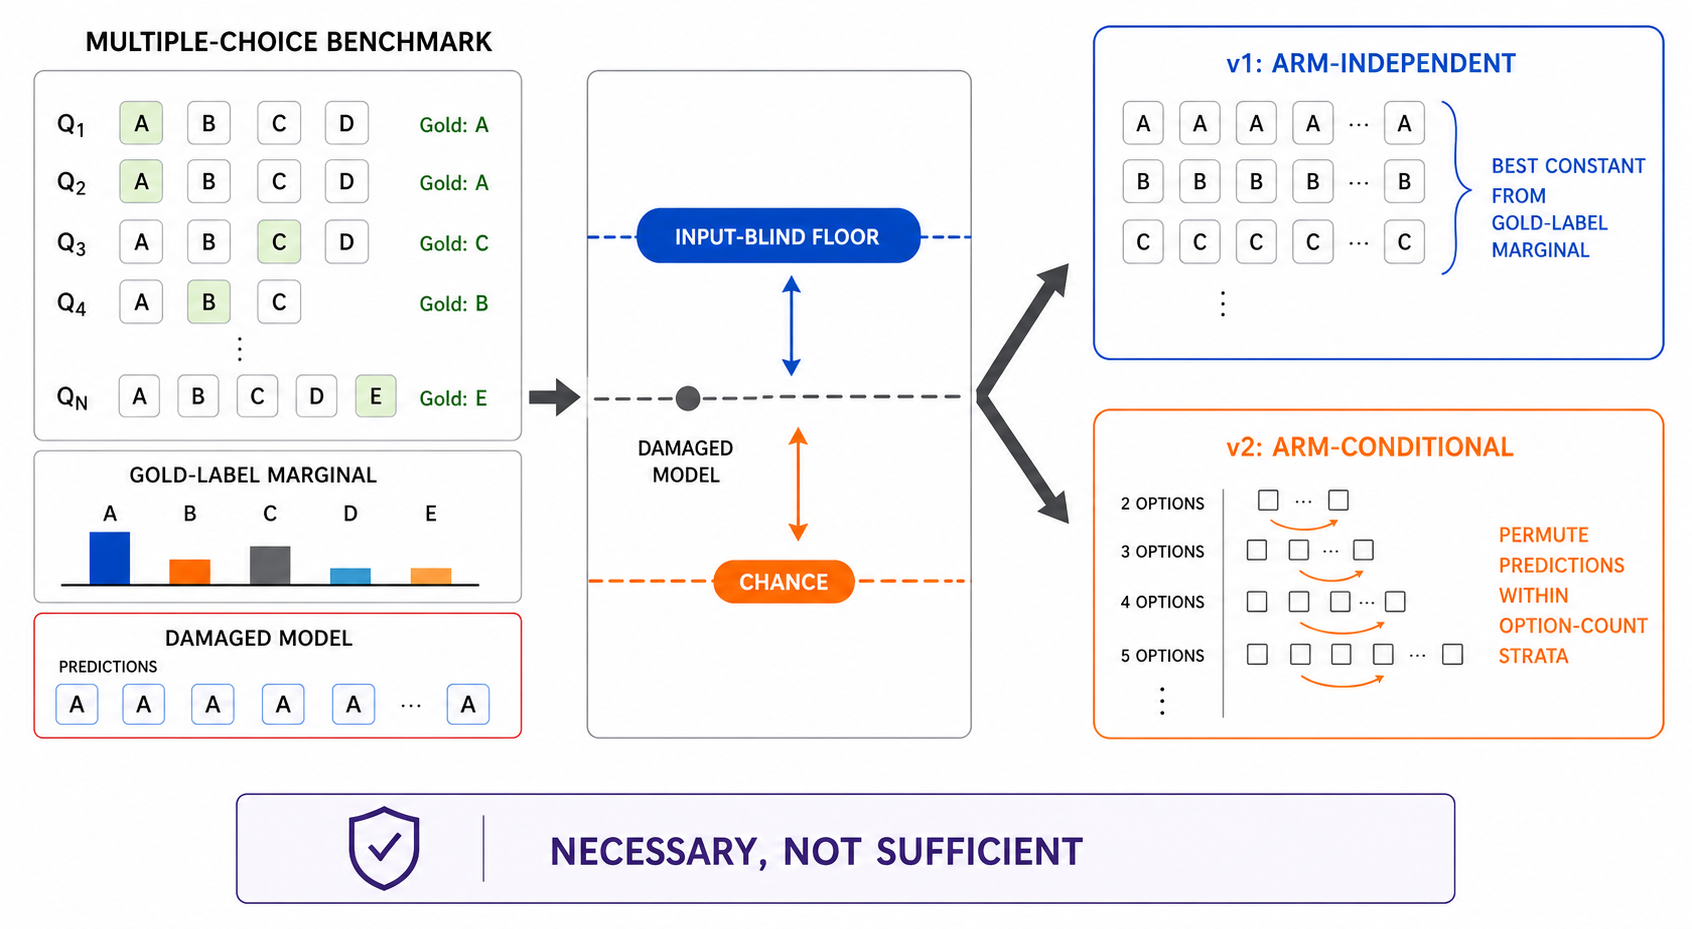
\includegraphics[width=\linewidth]{figures/teaser_candidate_r58_legible.png}
    \caption{Two construct-matched nulls. Arm-independent v1 uses the best constant under the gold-label marginal for comparability; arm-conditional v2 preserves legal option-count strata and the prediction marginal to test item-level information. Either is a reporting reference, not a logic gate, for construct validity.}
    \label{fig:construct-null-concept}
\end{figure}
\section{Introduction}

A recent multilingual evaluation reported that every tested model exceeded chance while none exceeded the benchmark's majority-class baseline \citep{arcon2026metalinguistic}. Printing both references exposed the discrepancy. A systematic construct-validity review of 445 language-model benchmarks provides 27 actionable checklist items but does not require reporting a null, chance level, or constant predictor \citep{bean2025measuring}. We address this operational gap: before comparing model arms, report whether the measured construct clears an appropriate input-blind reference. Figure~\ref{fig:construct-null-concept} previews the two references needed for interface comparability and arm-specific item-level information.

For a letter-valued multiple-choice construct, the floor is the most accurate constant letter under the benchmark's empirical gold marginal. For content likelihood, an analogous input-blind heuristic can exploit option length. Neither reference need equal nominal chance. An arm can therefore appear above chance while conveying no more usable signal through the measured interface than a constant predictor, especially after structural damage, when option-token selection bias \citep{zheng2024selectors} can dominate the argmax even if some content knowledge remains.

We study null calibration as a \emph{measurement protocol}, not a new multiple-choice interface or debiasing algorithm. Majority-class baselines for MCQA already exist \citep{balepur2024artifacts}; letter-versus-content formulations are established \citep{gu2025olmes,cho2026choices}; constant outputs can game automatic judges \citep{zheng2025cheating}. Our contribution is to make the construct-appropriate input-blind null an explicit pre-comparison reporting check, quantify the choices hidden in its definition, and separate two questions that require different references:

\begin{enumerate}[leftmargin=*,nosep]
    \item \textbf{Is the interface valid for arm comparison?} Use an arm-independent best-constant floor.
    \item \textbf{Does this particular arm carry item-level information?} Use an arm-conditional permutation null that preserves the arm's prediction marginal.
\end{enumerate}

This distinction prevents two opposite errors. Nominal chance can credit a literal constant emitter as competent, whereas the best-constant floor can assign different deltas to equally uninformative emitters that collapse onto different letters. The first error motivates our headline floor; the second motivates read-out v2 and its algebraic constant-collapse invariance.

Our evidence uses ten target constructs plus Winogrande as a negative control, four base-model families, letter and content likelihood interfaces, and structurally damaged arms. Our findings:

\begin{itemize}[leftmargin=*,nosep]
    \item The null is not ``chance,'' and the floor must itself be calibrated against a null the construct can \emph{realise}. Our first MMLU-Pro calibration violated that requirement. The corrected construct-level estimates and verdicts are reported in Table~\ref{tab:nulls}; only MMLU and BoolQ support a quantitative above-balanced-null claim.
    \item Content floors are not dataset constants unless their tie convention, length unit, and tokenizer are fixed. Table~\ref{tab:conventions} reports the measured reversals and spans; Section~\ref{sec:legality-aware-null} records the separate option-count correction.
    \item At MMLU-scale power, the conventional chance reference materially overstates the damaged-arm count. Table~\ref{tab:headline-reference} puts the chance and best-constant comparisons under matched point-estimate and interval standards; Appendix~\ref{app:designated} reports the exceptions and power limits.
    \item The permutation null makes every pure constant emitter score exactly zero, re-sorts rather than uniformly shrinks the read-out, and reveals intact Llama-2-7B as a weak MMLU-Pro anchor (Tables~\ref{tab:v2-resort} and~\ref{tab:v2-full}).
    \item Full-fp32 evaluation removes the exact-tie mechanism without recovering accuracy; the compact diagnostic audit in Table~\ref{tab:diagnostic-contrasts} separates that result from the integrity repairs.
\end{itemize}

The floor comparison is deliberately one-directional: failure withholds an above-reference label from a score used in an arm comparison, whereas passing does not certify that the benchmark measures the intended capability. \citet{feng2019misleading} construct a dataset in which a partial-input baseline is at chance while artifacts remain exploitable; one input-blind check cannot enumerate every validity threat.

\section{Related Work}

\paragraph{Input-blind and constant baselines.}
\citet{balepur2024artifacts} define a majority-class baseline for letter MCQA and recommend stronger-than-chance references; their object is dataset cheatability under a black-box generative setup, ours a per-arm gate for likelihood-scored constructs. The distinction is operational: their invalid-output analysis imputes either 0.0 or 0.25 on MMLU, while the construct's best-constant letter value is 0.2689. \citet{zheng2025cheating} use ``null model'' for crafted constant responses that adversarially exploit an LLM judge --- an attack optimized against a judge, whereas ours is a reference derived from benchmark statistics, requiring no attacker. The metalinguistic preprint motivating our opening reports the above-chance/below-majority pattern descriptively on one new benchmark, without turning it into a pre-comparison protocol \citep{arcon2026metalinguistic}.

\paragraph{Selection bias and MC interfaces.}
Letter preference is not a new observation. \citet{zheng2024selectors} identify selection and token bias and propose PriDe, which estimates an option-ID prior from permuted contents. PriDe fixes the predictor; null calibration fixes the reference line. Even after prediction debiasing, reporting only against chance can leave the benchmark's gold-marginal floor unreported. We therefore do not reject permutation controls on cost grounds --- they are a useful and potentially inexpensive diagnostic, answering whether predictions should be corrected, while our arm-independent floor answers whether the resulting interface score is comparable across arms.

OLMES standardizes both multiple-choice formulation (MCF) and cloze formulation (CF), then uses the better score per task and model \citep{gu2025olmes}; this is not a size-keyed rule. Its reference discussion is nevertheless framed around a random baseline rather than a measured label-marginal floor, so the max rule can select an interface without testing whether that interface clears an input-blind reference. Our ARC-Easy result shows CF rescuing an at-floor letter read-out; MMLU shows that an interface swap need not do so. \citet{cho2026choices} independently study symbols, cloze, and hybrid formats and propose a new question-sensitive score. We do not claim the interface contrast; our method instead gates whichever construct is reported.

\paragraph{Length-based scoring.}
Length-normalized likelihood can over-correct and its token-based form is tokenizer-dependent \citep{oostermeijer2026length}, so we claim no generic length sensitivity or tokenizer dependence of the scoring rule. We show the \emph{induced input-blind floor} inherits these choices: its value changes with tie convention, character versus continuation-token length, and tokenizer. OLMES's observation that tokenizer dependence may be irrelevant when ranking options for one fixed model and tokenizer is compatible with ours; our scope is cross-model comparison of the reference itself.

\paragraph{Nulls as interpretive controls.}
Our arm-conditional read-out v2 is a chance-corrected agreement statistic: $\Delta_{\mathrm{perm}}$ equals the numerator of Cohen's $\kappa$ \citep{cohen1960kappa} within option-count strata, and the constant-emitter zero we rely on is that literature's standard property, not a new result. We claim only the stratification by variable option count and the statistic's use as a pre-comparison gate.

Control tasks and selectivity can reverse conclusions about which representation layer is informative \citep{hewitt2019probes} --- the closest structural precedent, their null randomizing supervision for a probe while ours removes input dependence from an MC construct. \citet{ding2021grounding} similarly motivate sensitivity and specificity tests for representation similarity. Finally, \citet{bean2025measuring} provide the construct-validity vocabulary and a broad benchmark checklist. We position null calibration as the missing operational item, not as the invention of construct validity.

\section{Null-Calibrated Measurement}

Let a benchmark have items $i=1,\ldots,n$, gold answers $y_{i}$, and a scored interface producing predictions $\hat{y}_{i}$, with empirical accuracy
\begin{equation}
    \mathrm{acc}=\frac{1}{n}\sum_{i=1}^{n}\mathbf{1}[\hat{y}_{i}=y_{i}].
\end{equation}

\subsection{Read-out v1: the arm-independent interface floor}

For a letter construct with legal labels $\mathcal{L}$, define the input-blind constant family $h_{L}(x)=L$. The construct floor is
\begin{equation}
    f_{\mathrm{const}}=\max_{L\in\mathcal{L}}\frac{1}{n}\sum_{i=1}^{n}\mathbf{1}[y_{i}=L].
\end{equation}
The v1 statistic is $\Delta_{\mathrm{floor}}=\mathrm{acc}-f_{\mathrm{const}}$. Because $f_{\mathrm{const}}$ depends only on the evaluated item set, every arm is compared to the same reference --- arm independence is essential, or arm-to-arm comparisons could change merely because the null changed with the arm.

For content likelihood, we use an input-blind longest-option family, whose prediction depends solely on option length but is not fully specified until a tie convention and length unit are fixed; token-based variants also require a tokenizer. Section~\ref{sec:nulls} treats these as part of the construct.

Our decision rule is intentionally asymmetric: failing the floor withholds the above-reference label from any claim that the interface expresses arm-specific capability above the strongest constant reference, while clearing it passes one necessary test but leaves artifacts no single null enumerates \citep{feng2019misleading}.

\paragraph{Why the floor is the achievable constant.}
The operative reference is the \emph{literal observed floor} $f_{\mathrm{const}}=\max_L(\mathrm{count}_L/n)$, not the balanced expectation $\mathbb{E}[\hat f]$, for a decision-theoretic reason: the realized construct must beat the best input-blind score \emph{actually attainable on this item set}, not the score a balanced benchmark of identical size would have delivered. The literal floor is the maximum-marginal constant a realizable interface could have reached by construction; any null calibrated to a uniform marginal scores a different, legal-but-unrealisable experiment against that construct (classically, the weighted-$\kappa$ corollary collapses to $1/k$ iff the marginal is uniform \citep{cohen1960kappa,brennan1981kappa}). The residual winner's-curse gap $f_{\mathrm{const}}-\mathbb{E}[\hat f]$ ($0.273$ pp on MMLU-Pro) is disclosed side-by-side in Table~\ref{tab:mmlupro}, so the reader sees both the baseline that was actually achievable and the selection-biased expectation the plug-in preserves.

\subsection{Read-out v2: an arm-conditional independence null}
\label{sec:v2}

The v1 floor asks whether an interface is suitable for mutually comparable arm scores; it is not collapse-invariant as a competence statistic. On the full MMLU-Pro item set, always-A, always-E, and always-J contain the same item-level information---none---yet receive unequal v1 deltas because the gold marginals are non-uniform (Table~\ref{tab:two-nulls}). The separate ten-letter implementation self-test below conditions each letter on items where it is legal.

For the arm-specific question, we preserve the arm's own prediction multiset and remove its alignment with items. MMLU-Pro has variable option count, so permutations are uniform \emph{within} \texttt{n\_opt} strata $s$. With $n_{s}$ the stratum size and $c^{\mathrm{pred}}_{s,L}$, $c^{\mathrm{gold}}_{s,L}$ the prediction and gold counts,
\begin{equation}
\widehat{\mathrm{acc}}
=\mathbb{E}[\mathrm{acc}\mid \hat{\boldsymbol y}\ \text{permuted within }s]
=\sum_s\frac{1}{n n_{s}}\sum_L c^{\mathrm{pred}}_{s,L}c^{\mathrm{gold}}_{s,L},
\end{equation}
and
\begin{equation}
    \Delta_{\mathrm{perm}}=\mathrm{acc}-\widehat{\mathrm{acc}}.
\end{equation}

\paragraph{The statistic is decades old; only the varying-$k$ stratification and its use are ours.}
$\Delta_{\mathrm{perm}}$ is the \emph{numerator} of Cohen's $\kappa$ within \texttt{n\_opt}
strata: with $p_o=\mathrm{acc}$ and $p_e=\widehat{\mathrm{acc}}$, $\kappa=(p_o-p_e)/(1-p_e)$,
hence $\Delta_{\mathrm{perm}}=\kappa\,(1-p_e)$ identically --- verified to printing precision in
all 27 cells of Table~\ref{tab:v2-full}. We claim neither this statistic nor the collapse
identity below as new: that chance-corrected agreement vanishes for a constant rater is the
textbook property, since $p_o=p_e$ there. That a chance term should depend on how many options
an item offers likewise long predates this work
\citep{bennett1954communications,brennan1981kappa,frary1988formula,brenner1996weightedkappa,%
devries2008pooledkappa}, and we claim none of it: neither correcting for option count, nor treating
$p_e$ as a methodological decision, nor noting that $\kappa$-family statistics depend on $k$. Those
works assume a single global $k$; what we are not aware of there, and do claim, is (i) a null in
which $k$ \emph{varies item to item} ($\texttt{n\_opt}\in\{3,\dots,10\}$, eight strata here), the
permutation confined within strata so a letter illegal for an item can never be credited to it, and
(ii) use of the quantity as an \emph{arm-conditional pre-comparison gate} with an explicit
materiality bar rather than as an agreement score. We report $\Delta_{\mathrm{perm}}$ rather than
$\kappa$ to keep it on the v1 floor's percentage-point scale, which is what makes the two nulls
directly comparable (Table~\ref{tab:two-nulls}). Appendix~\ref{app:priorart} states that boundary
claim by claim; its footprint is the $36$ items below.

\paragraph{Constant-collapse identity.}
For a pure always-$L$ emitter, $P(\hat{y}=L')=\delta_{L'L}$. Writing $m_{L'}$ for the relevant gold marginal,
\begin{equation}
\widehat{\mathrm{acc}}
=\sum_{L'}\delta_{L'L}m_{L'}
=m_{L}
=\mathrm{acc},
\qquad
\therefore\quad \Delta_{\mathrm{perm}}=0.
\end{equation}
This is an algebraic identity for every legal collapse letter, not an empirical regularity: it is the $\kappa=0$ property specialised to our stratified estimator, and the implementation asserts zero to below $10^{-12}$ for all ten letters. The loophole ``collapse onto a different letter'' is therefore closed by construction.

The two nulls must not be conflated, and their ordering is weaker than it first appears. Unstratified, $\sum_L p_{L}m_{L}\leq\max_Lm_{L}$ places the v2 null at or below the v1 best-constant floor; within-stratum permutation instead yields a bound that can dominate $f_{\mathrm{const}}$ when stratum argmaxes differ. Appendix Table~\ref{tab:ordering-audit} gives the exact combinatorial gap, empirical count, binding cell, and legal counterexample. The ordering holds for the measured cells but becomes a theorem only under a regularity condition we can state and not assume. \textbf{Passing v2 must never be described as clearing the paper's floor.}

Uncertainty uses 10,000 paired bootstrap resamples with $\widehat{\mathrm{acc}}$ recomputed inside each, cross-checked against 10,000 within-stratum permutations; both use seed 7 and must agree at $\alpha=0.05$. Significance is not enough at $n=12032$, so we define

\paragraph{Reference-choice reporting rule (operative).}
\paragraph{Operative calibration reference.} Throughout the paper the operative calibration reference for per-cell `above floor' / `at floor' / `below floor' verdicts is the \emph{literal observed best-constant floor} $f_{\mathrm{const}}=\max_L(\mathrm{count}_L/n)$ ($1403/12032=0.116606$ on MMLU-Pro). Table~\ref{tab:headline-reference} consolidates the matched-standard headline counts, and Table~\ref{tab:mmlupro} prints every MMLU-Pro cell; all are \emph{defined against the observed floor}. Where a count against $\mathbb{E}[\hat f]$ differs, both figures are printed. The selection-aware joint resample that would also vary the winning letter is \emph{not run} here (items unavailable this run; plug-in/Wilson intervals only). Any future re-judging that treats the winner letter as random must re-issue the counts and must not silently re-use these figures.

\paragraph{Frozen sensitivity surface \texorpdfstring{$\mathbb{E}[\hat f]$}{E[f-hat]}.} The legality-aware balanced-null expectation always accompanies the literal reference in Table~\ref{tab:mmlupro} but enters verdicts only as a \emph{frozen supplement/sensitivity surface}, never as a replacement. Appendix Table~\ref{tab:reference-anatomy} aligns the cells separating the references: sign flips do not automatically change interval verdicts, one healed OLMo-2 cell straddles the literal floor, and the clear-both comparator remains distinct. Where aggregate counts differ, both are printed in the corresponding tables rather than repeated here.

\begin{equation}
\text{\texttt{recovery\_fraction}}=\frac{\Delta_{\mathrm{perm}}}{\Delta_{\max}},
\end{equation}
with $\Delta_{\max}$ the best alignment achievable by reassigning the observed prediction multiset subject to each item's legal option count, and require at least 0.10 times the same-family intact anchor for a material signal. If the intact anchor fails that cutoff, relative claims are blocked. Appendix Table~\ref{tab:materiality-diagnostics} reports the full threshold sweep; membership is unchanged in the intended operating neighbourhood and only the lowest sensitivity boundary admits three additional cells.

\paragraph{Pre-registration status.}
The v2 rule, gates, stratification, and materiality constant were committed before re-judging the existing cells and before future unscored milestones. The 27 numbers here are nevertheless post-hoc by construction: those cells had already been scored, and the designer had already seen the shape of the collapse defect. We therefore present v2 as a pre-registered rule for future read-outs and a transparent post-hoc re-analysis of the existing cells.

% --- ICLR 2026 page budget ---------------------------------------------------
% Section 4 "Four Under-Specifications of the Reference" is DEVELOPED in the
% appendix (sections/03b_nulls.tex, \input from 09_appendix.tex, i.e. after the
% bibliography). The main text keeps a self-contained summary that names all four
% degrees of freedom and states every headline number, so a reader who never opens
% the appendix still learns what the four under-specifications are. Nothing was
% deleted. Provenance + measured page budget: the distributed Appendix.
% -----------------------------------------------------------------------------
\subsection{Four under-specifications of the reference}
\label{sec:nulls}

A content floor is not a dataset constant. Four independent choices must be printed with the score: the tie convention, the length unit, the tokenizer, and --- when option count varies --- the definition of chance. In our audit, tie handling can reverse an ARC-Challenge verdict, and the extreme-convention sensitivity span on MMLU-Pro is much larger than the operative span among defensible conventions; changing the length unit or tokenizer also moves the floor by more than the effects under study. Nominal and item-averaged chance likewise disagree on MMLU-Pro. Tables~\ref{tab:nulls} and~\ref{tab:conventions} place the exact floors, tie rates, gaps, sensitivity endpoints, and calibrated verdicts in aligned columns; Appendix~\ref{app:nulls} develops each choice and its provenance. Jointly, the four define a token content floor as a property of $(\text{dataset},\text{convention},\text{unit},\text{tokenizer})$. The letter floor is exempt: it depends only on the item set's gold-label marginal.

\section{Experimental Setup}
\label{sec:setup}

\paragraph{Benchmarks and constructs.}
We evaluate letter constructs on MMLU~\citep{hendrycks2021measuring}, ARC-Challenge and ARC-Easy~\citep{clark2018think}, OpenBookQA~\citep{mihaylov2018openbookqa}, CommonsenseQA~\citep{talmor2019commonsenseqa}, PIQA~\citep{bisk2020piqa}, MMLU-Pro~\citep{wang2024mmlupro}, and Winogrande~\citep{sakaguchi2020winogrande} as a negative control; BoolQ~\citep{clark2019boolq} supplies an additional binary label floor. Content-side longest-option constructs use MMLU, MMLU-Pro, and the five non-MMLU evidence tasks, Winogrande again only as a control. The inventory is ten constructs plus the control; OpenBookQA content is reported under both character and token units rather than counted twice.

\paragraph{Models and structural damage.}
The four families are OLMo-2-7B~\citep{groeneveld2024olmo}, Llama-2-7B~\citep{touvron2023llama2}, Llama-3-8B~\citep{grattafiori2024llama3}, and Qwen3-8B-Base~\citep{yang2025qwen3}. OLMo-2 arms are prune-then-heal checkpoints, including \texttt{keep8}, \texttt{keep10}, \texttt{keep12}, \texttt{keep14}, and \texttt{shortgpt16}. Non-OLMo damage is evaluation-time front-$N$ truncation: the intact base is loaded and its layer list replaced by the first $N$ blocks, with no fresh block, optimizer, gradient, healing, or damaged checkpoint --- a regime confound, not a clean family contrast, and every joint table labels it. Qwen3's 36 layers against the others' 32 make \texttt{k8} retain 22.2\% rather than 25.0\%.

\paragraph{Interfaces and scoring protocol.}
The letter prompt is the content prompt with the labelled option body inserted before \texttt{Answer:}; the letter interface scores the continuations `` A'', `` B'', and so forth, while the content interface omits the labelled body and scores option text. Scoring is likelihood-based throughout: summed token log-probability over each candidate continuation, then argmax. There is no sampling, no decoding, and no regex over generated text.

All results use \texttt{chat\_template = False}: the evaluated systems are base language models with no supervised fine-tuning and no reinforcement learning from human feedback, so applying a chat template would be an unfair and non-comparable measurement. We also use \texttt{add\_bos = 0}, \texttt{desc\_style = none}, fp32 master weights with bf16-autocast forward, and batch size 48. MMLU-Pro cross-family runs use maximum length 2048; every final cell has zero truncation. Numbers here are all from the corrected launch; the \texttt{protocol.max\_len=1536} field inside the per-cell MMLU-scale record is retained for provenance (Appendix~\ref{app:mmlupro-and-resort}).

\paragraph{Statistics and integrity.}
For deterministic per-item null predictions we report 10,000-resample paired-bootstrap intervals and two-sided mid-$p$ values with seed 7, plus exact McNemar tests; v2 additionally uses 10,000 within-stratum permutations. Every cell requires shard indices exactly $\{0,\ldots,7\}$, expected cardinality, zero duplicate IDs, zero NaNs, zero truncations, and \texttt{chat\_template is False}; partial merges raise an error.

\paragraph{Power design.}
The five smaller evidence benchmarks cannot resolve every effect of interest, so null results are never interpreted without the power table (Table~\ref{tab:power}, Appendix~\ref{app:designated}).
MMLU-Pro supplies $n=12032$ and makes all 21 letter-floor cells capable of detecting MMLU's $-1.389$-point reference effect, with 95\% half-widths from 0.083 to 0.968 points.

\paragraph{Designated damaged cells, and multiplicity.}
Every denominator below is over \emph{designated damaged} cells: all five OLMo-2 prune-then-heal arms and all four truncation rungs of each non-OLMo family, giving 17 MMLU-Pro cells and 85 off MMLU, with Winogrande the sole excluded control. The designation is fixed by construction, never by a measured score, and is identical in every denominator; Appendix~\ref{app:designated} records that an earlier version narrowed it on MMLU-Pro without saying so. We report per-cell $\alpha=0.05$ decisions with no family-wise correction, so headline counts are counts of per-cell decisions rather than simultaneously valid claims; the conclusions rest on the aggregate's direction and on the regime-and-depth pattern organising its exceptions, not on one cell.

\section{Results and Analysis}

\subsection{Wrong-null verdict flips at MMLU-scale power}
\label{sec:flips}

MMLU-Pro provides the cleanest test. Table~\ref{tab:headline-reference} aligns the chance and best-constant counts under matched point-estimate and interval standards; Table~\ref{tab:mmlupro} in Appendix~\ref{app:mmlupro-and-resort} gives the per-cell values. The reference changes the damaged-arm interpretation, but not every cell moves, so we retain the exact counts rather than claim a universal categorical flip.

\paragraph{Both sides of the flip, held to one standard.}
Those counts were initially asymmetric in evidentiary standard: the floor side carried an interval and a test, whereas ``above chance'' was a bare point comparison. Because both references are deterministic functions of the evaluated item set, the same paired bootstrap can be applied to each side.

\begin{table}[!htbp]
\centering
\scriptsize
\setlength{\tabcolsep}{3pt}
\begin{tabular}{@{}lcc@{}}
\toprule
Scope and standard & Above chance & Above best-constant floor \\
\midrule
MMLU-Pro non-OLMo, point estimate & 10/12 & 3/12 \\
MMLU-Pro non-OLMo, CI$_{95}$ excludes 0 & \textbf{3/12} & \textbf{1/12} \\
MMLU-Pro non-OLMo, BH/Bonferroni at 0.05 & 0/12 & 0/12 \\
Off-MMLU designated OLMo-2 heal cells (25), point est. & 20/25 & 9/25 \\
Off-MMLU designated non-OLMo cells (60), point est. & 25/60 & 4/60 \\
Off-MMLU designated non-OLMo cells (60), CI$_{95}$ excl.\ 0 & --- & 0/60 \\
\bottomrule
\end{tabular}
\caption{\textbf{Calibrating the reference sharply reduces the advertised damaged-arm count.}
The first two rows compare matched point-estimate and paired-bootstrap standards; the third records the
multiplicity result under either stated correction; the final three show
the off-MMLU replication by regime. `Above chance' uses $\mathrm{mean}(1/\texttt{n\_opt})$.
Exact cells and power limits in Tables~\ref{tab:mmlupro} and~\ref{tab:power}. The paired bootstrap
conditions on the observed winning letter; the selection-aware joint resample is \textbf{not run}.}
\label{tab:headline-reference}
\end{table}

The symmetric interval comparison is about one third the size suggested by the asymmetric point-estimate comparison. This does not weaken the reporting rule; it removes an evidentiary mismatch and shows why both the reference and its uncertainty must be stated.

Table~\ref{tab:headline-reference} shows that every interval-level off-MMLU clear belongs to the OLMo-2 rows and aligns the chance, point-floor, and interval-floor counts without repeating them in prose. The item-average convention is operative; the nominal convention would restore the pre-calibration chance-side reading on the MMLU-Pro rows. A joint-resample re-issue is the natural follow-up and must not re-use these counts.

Two qualifications belong with this comparison, both quantified in Appendix~\ref{app:analysis-mult}. McNemar's test does not transfer to a non-binary chance reference, and neither side retains an individual cell after multiplicity correction. The aggregate chance-side count remains unlikely under a global null, so we read it as evidence that the chance side is not uniformly null, not as simultaneously valid per-cell claims.

The result is strong but not universal: 15/17 cells are at or below the floor, and the two exceptions differ in kind. Table~\ref{tab:mmlupro} shows that \texttt{qwen3\_8b\_base/k14} is statistically real but below the materiality gate, whereas OLMo-2 \texttt{shortgpt16} clears its floor decisively. The latter retains more of the stack than any \texttt{keepN} rung, so the floor test does not indiscriminately reject damaged arms (Appendix~\ref{app:designated}).

\paragraph{Materiality is stable against its own threshold.} Figure~\ref{fig:gate-materiality} plots the half-width diagnostic and signed $\Delta_{\mathrm{perm}}$ against the recovery fraction for every cell. The intact Llama-2 anchor fails the precondition, so that family's relative-recovery stack is blocked; Table~\ref{tab:v2-full} supplies the numerator intervals, while $\Delta_{\max}$ is deterministic. Appendix Table~\ref{tab:materiality-diagnostics} reports the full threshold sweep and per-cell diagnostics: the material set is unchanged throughout the intended operating range, and only the lowest sensitivity boundary admits additional cells. Llama-2 remains excluded throughout because its intact anchor fails, not because of post-hoc selection. The table is recomputed from the frozen \texttt{heal\_readout\_v2\_permutation\_null.json} record by \texttt{code/emit\_materiality\_sweep.py}.

The small-benchmark replication contains literal constant emitters that sit on the optimal constant while appearing above chance: the final rows of Table~\ref{tab:headline-reference} show the aggregate supersession of the advertised damaged-arm count. Every surviving above-floor case is a healed \textsc{OLMo-2} arm retaining at least 14 layers; no shallower healed arm or truncate-only arm \emph{significantly} clears its floor. Margins and per-cell counts in Tables~\ref{tab:headline-reference} and~\ref{tab:offmmlu-cells}. Because \textsc{OLMo-2} is the only healed family, this remains a property of that ladder, not a family effect. Appendix~\ref{app:offmmlu} reports the exact constant-emitter, depth, and power counts.

\subsection{Read-out versus retained knowledge}

A floor-level letter score does not imply all task-relevant competence is gone. The ARC-Easy contrast in Table~\ref{tab:diagnostic-contrasts} shows an arm that can rank contents but cannot express that knowledge through the damaged letter interface. Conversely, healthy models often favor letters, so ``content is the fair interface'' generalises no better.

The residual-fraction effect is likewise construct-specific: chance inflates it on OpenBookQA but slightly deflates it on PIQA and ARC-Easy. Null calibration is therefore not a one-way correction; the exact ratios are recorded in Appendix~\ref{app:offmmlu}.

\begin{table}[!htbp]
\centering
\small
\setlength{\tabcolsep}{3.5pt}
\begin{tabular}{@{}p{0.19\linewidth}p{0.24\linewidth}p{0.25\linewidth}p{0.23\linewidth}@{}}
\toprule
Diagnostic & Baseline/read-out & Intervention/contrast & Takeaway \\
\midrule
ARC-Easy \texttt{keep8} & letter 0.2584; floor 0.266414 & content 0.6460; gap $+38.76$ pp & content survives the damaged letter interface \\
Qwen3 \texttt{k8} & v1 $-0.881$ pp ($p=0.0362$) & v2 $-0.139$ pp ($p=0.0964$) & below-floor competence label dissolves \\
Llama-2 \texttt{k8} & v1 $-0.914$ pp ($p=0.0168$) & v2 $-0.416$ pp ($p=0.1002$) & below-floor competence label dissolves \\
OLMo-2 \texttt{keep8}, MMLU & 4,303 bf16 ties; 2,532/14,042 argmax changes & fp32 has zero ties; $\Delta$accuracy $=-0.0015$ & numerical precision does not recover accuracy \\
Qwen3 \texttt{k14} & shipped BH family: 27 cells, $q_{\mathrm{BH}}=0.0297$ & damaged-only family: 23 cells, $q_{\mathrm{BH}}=0.0759$ & multiplicity-corrected downgrade dissolves \\
\bottomrule
\end{tabular}
\caption{\textbf{Representative interventions separate interface failure, arm-conditional signal, and numerical precision.} Full intervals and multiplicity-adjusted results in Tables~\ref{tab:v2-resort} and~\ref{tab:v2-full}.}
\label{tab:diagnostic-contrasts}
\end{table}

\paragraph{V2 re-sorts the 27-cell read-out.}
Under v1, two MMLU-Pro cells are significantly below the best-constant floor; under v2 the below-null count is zero (Table~\ref{tab:diagnostic-contrasts}). V2 is not uniformly conservative: it downgrades \texttt{qwen3/k14} and upgrades \texttt{olmo2/keep14}. The \texttt{qwen3/k14} downgrade survives only under the originally shipped 27-cell BH family and not the pre-declared 23-cell damaged-only family, so we report it as an \emph{uncorrected per-cell observation}. V2 also exposes intact Llama-2-7B as a weak arm-conditional anchor, blocking relative-recovery claims for that family (Table~\ref{tab:v2-resort}).

\begin{figure}[H]
\centering
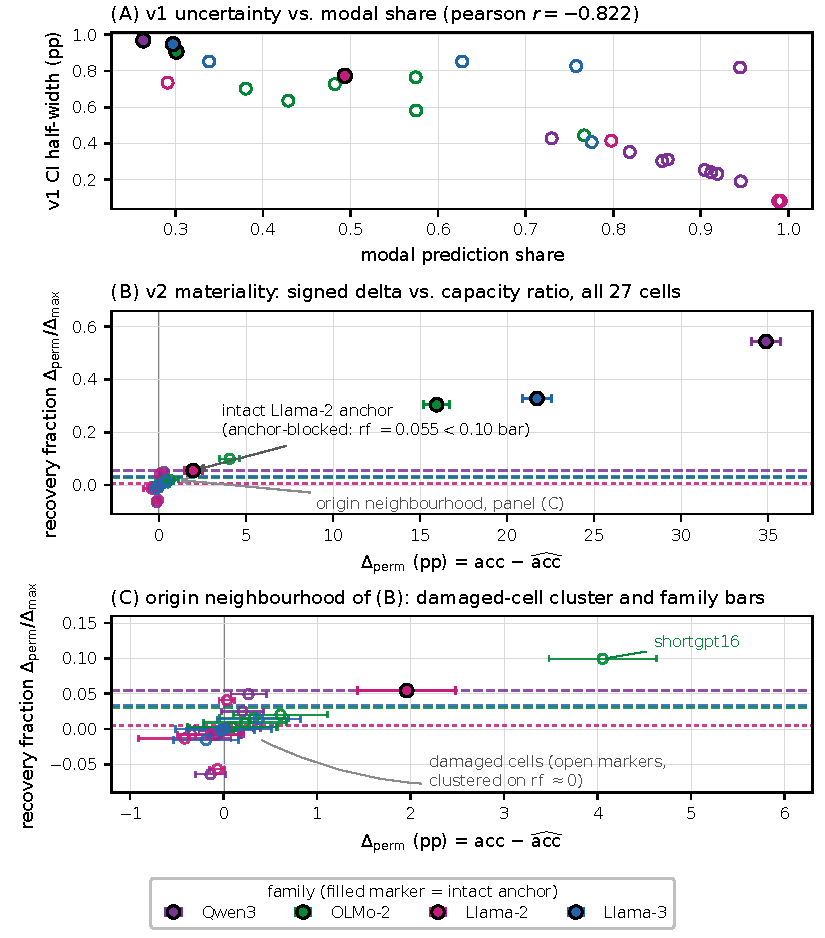
\includegraphics[width=\linewidth]{figures/fig_gate_materiality.pdf}
\caption{\textbf{Quantitative evidence for the gate and its materiality bar (27 cells).}
\textbf{(A)} v1 CI half-width against modal-prediction share (pearson $r=-0.822$;
Table~\ref{tab:v2-full}). \textbf{(B)} signed $\Delta_{\mathrm{perm}}$ against
$r_f=\Delta_{\mathrm{perm}}/\Delta_{\max}$ and the pre-registered family bar.
$\Delta_{\max}$ is deterministic; all 27 rows are in Table~\ref{tab:materiality-diagnostics}.}
\label{fig:gate-materiality}
\end{figure}

\section{Discussion}

\textbf{Reporting rule.} Report the construct-appropriate input-blind reference, its uncertainty, and its role beside each arm comparison. V1 is arm-independent and addresses interface comparability; v2 is arm-conditional and addresses item-level alignment. Neither certifies construct validity. \textbf{Empirical scope.} On MMLU-Pro, 15/17 designated damaged cells are at or below their best-constant floor despite exceeding chance at the point-estimate level (Table~\ref{tab:mmlupro}). Off MMLU, interval-level clearance is confined to healed OLMo-2 arms retaining at least 14 of 32 layers. Because regime, family, depth, corpus, and exposure are confounded, this describes the measured ladder rather than a universal damage law (Appendix~\ref{app:ledger}).


% --- ICLR 2026 page budget -------------------------------------------------
% The Ethics Statement and the Reproducibility Statement are EXCLUDED from the
% 9-page main-text limit by the ICLR 2026 Author Guide, but only read as excluded
% when they do not sit inside the main text. Both are therefore emitted after the
% bibliography. Source: ICLR 2026 Author Guide, page-limit clause.
% Section 7 (Limitations) is emitted after the bibliography beside the
% Ethics Statement, at the position the author guide treats as page-exempt,
% so that Sections 1-6 still land on the 9-page main-text budget. Patch
% A-L0 in paper/patch_plan.md (C1, 2026-08-21).
% ---------------------------------------------------------------------------
% P5_MAIN_TEXT_END
\label{p5:main-text-end}
\bibliography{refs}
\bibliographystyle{iclr2026_conference}

\section{Ethics Statement}

This work uses existing benchmark records and base-model checkpoints, collecting no human-subject data and making no deployment claim. The main ethical risk is epistemic: a poorly calibrated reference can make a damaged or degenerate system appear capable, distorting model comparisons and downstream decisions. We mitigate by publishing the null definition, uncertainty, power, integrity checks, counterexamples, and a flat retraction ledger, and by not treating a floor pass as certification (untested artifacts may remain).

The experiments consumed substantial accelerator resources; the manuscript itself adds none. Our recommended nulls use only existing labels, option metadata, and prediction records, so they can usually be added with negligible compute relative to model evaluation.

\section*{Reproducibility Statement}

Every quantitative claim in this paper is bound to a machine-readable record, and the
binding is checked mechanically rather than by hand. A checker walks the marked numerals in the
source and requires each to be either an exact match to a value in the evidence set, a
correct rounding of one, or a stated difference of two. Table~\ref{tab:repro-audit} aligns the
coverage counts, the sole checker-scope flag, and the wider scan. The flag is not a transcription
error: the Qwen3 \texttt{k8}/PIQA accuracy in Table~\ref{tab:offmmlu-cells} matches its own per-cell
record, while the checker treated the floor-adjacent literal as a floor. The same table records
which statistics are emitted from per-item prediction records rather than transcribed, so a reader
who re-runs the emitters obtains the printed tables or a diff.

\begin{table}[H]
\centering
\small
\setlength{\tabcolsep}{4pt}
\begin{tabular}{>{\raggedright\arraybackslash}p{0.22\linewidth} >{\raggedright\arraybackslash}p{0.27\linewidth} >{\raggedright\arraybackslash}p{0.41\linewidth}}
\toprule
Audit slice & Recorded result & Interpretation \\
\midrule
Marked prose values & 67 checked; 66 exact or correctly rounded; 1 flagged; 12 skipped; 0 uncovered & The sole flag is inspected below rather than silently waived. \\
Flagged literal & Qwen3 \texttt{k8}/PIQA accuracy 0.505441; construct floor 0.504897 & The checker applied a floor-adjacent rule to an accuracy field; the printed accuracy matches its per-cell record. \\
Wider source scan & 653 numerals; 0 unresolved & No unresolved literal remains in the expanded scan. \\
Generated statistics & Two nulls, winner's-curse calibration, stratified permutation, and power tables & Each is emitted from per-item records; rerunning yields the printed tables or a diff. \\
\bottomrule
\end{tabular}
\caption{\textbf{The reproducibility audit separates coverage from the single explained checker flag.} Counts come from \texttt{evidence/prose\_vs\_evidence\_check.json}; the compared Qwen3 values are retained side by side so the checker-scope mismatch is auditable without a numeric wall in prose.}
\label{tab:repro-audit}
\end{table}


The measurement protocol is fixed and reported in full in
Section~\ref{sec:setup}: \texttt{chat\_template = False}, \texttt{add\_bos = 0},
\texttt{desc\_style = none}, fp32 master weights with bf16-autocast forward, batch size 48,
and maximum length 2048 for the cross-family MMLU-Pro runs, with zero truncation asserted
per shard in every reported cell. The chat template is disabled deliberately and not for
convenience: the evaluated systems are base language models with neither supervised
fine-tuning nor RLHF, so applying a chat template would measure a different object.

Three properties of this study are load-bearing for reproduction and are stated here
rather than left implicit. First, the floor is a maximum over noisy label marginals and is
therefore upward biased even under exactly uniform labels; any attempt to reproduce a
floor-above-chance claim must reproduce that calibration, not only the point estimate.
Second, content-side floors are not a property of a dataset alone: they are determined
jointly by the tie convention, the length unit, and the tokenizer, so a reproduction that
fixes only the dataset will not recover our numbers. Third, the ordering between the two
nulls is a measured property of the reported cells under an explicitly stated regularity
condition, not an identity; we give the margin by which it holds and the construction that
violates it.

We also record what a reproduction will \emph{not} find. Claims that earlier drafts of this
work considered and that the evidence did not sustain are listed with their current status
in Table~\ref{tab:claims}, including six retracted and two prohibited numeric claims. That
ledger is part of the artifact: it exists so that a reader who encounters one of those
numbers elsewhere can see that we withdrew it and why.

\paragraph{Artifact availability.}
The complete evidence pack, build record, code, and frozen
sources of every table are attached as an anonymized supplementary archive to this
submission (paths resolve relative to the code-repository root as in Table~\ref{tab:integrity}). The
anonymisation gate covers the compiled PDF (\texttt{layout\_audit.json:anonymization});
the longer identifiers and file paths inside evidence JSON and code files resolve only
relative to the anonymized repository root, and contributor-identifying
verbatim lines in non-\texttt{.tex} inputs were scrubbed by \texttt{code/scrub\_artifact\_paths.py}
with a fail-closed post-pass verification (zero identifying literals remain). Every
numeric value in the paper is one of (i) emitted by a script in the archive from a frozen
input file, (ii) quoted from a public benchmark with its exact download checksum, or (iii)
a pure-arithmetic rewriting of (i)--(ii); none is introduced by hand into a table or
sentence. The numeral-checker run by \texttt{code/check\_prose\_vs\_evidence.py}
(and its dedicated table-level sibling) validates \emph{transcription fidelity} between
source manifests and the compiled PDF strings; it does \emph{not} verify the upstream
statistical computation itself (raw-data to statistics); that second layer is the
reproduction path documented above. The selection-aware joint bootstrap used for the
$\mathbb{E}[\hat f]$ calibrating-reference verdicts is \emph{not run} in this version
(per-item letter-level prediction shards are not in the release artifact; the
numbered floors and counts reported are therefore plug-in/Wilson intervals only, and any
future re-issue must re-run the selection step). The anonymous artifact registry lives
at \texttt{paper/SHA\_PIN\_R13.\{json,md\}} (frozen manuscript identifier and content
association), \texttt{paper/evidence/} (one JSON or CSV per evidence tag \textsf{E-A}
through \textsf{E-K} plus \textsf{E-CAL}), and \texttt{review/SEAL\_RETIREMENT\_REGISTRY.json}
(append-only lineage + successor replacement for the seal/identity sha of every
superseded build).


\appendix
\renewcommand{\thesection}{\Alph{section}}
% --- Limitations (appendix placement, R92 M9) --------------------------------
% LIMITATIONS, full version. Emitted AFTER the bibliography beside the Ethics
% Statement so that the 9-page main-text content budget (Sections 1-6) is
% untouched; the main text keeps no bridge. This is the same treatment the
% ICLR 2026 author guide gives the Ethics and Reproducibility statements and
% follows the aggregate's item-12 footnote that Limitations, if not
% exempt, must fit on the main pages. Provenance: patch_plan.md A-L0, C1,
% 2026-08-21.

\section{Limitations}
\label{sec:limitations}

\paragraph{Character-unit reconstruction.}
The OpenBookQA character floor, added after the original audit flagged an evidence hole, is now recomputed from raw parquet and passes a 12/12 character/token self-test; the narrower remaining limitation is that character values are reconstructed from raw option text rather than stored per-item in the scored records. Item matching to the token leg therefore follows the shared loader and self-test, not a stored character-count column. The convention of excluding the continuation's leading space was explicit; including it yields the identical 0.363500 value.

\paragraph{One family at one depth; unmatched healing corpora.}
The prospective healed comparison has unmatched family, depth, corpus, and exposure. Table~\ref{tab:limitations-audit} places those quantities on aligned rows; the Qwen3 arm also cannot consume OLMo-2-token Dolmino, whose raw text is on neither disk. The design therefore supports neither a depth gradient nor a family contrast.

\paragraph{Regime, pooling, and the planned causal contrast.}
Tables mixing truncate-only non-OLMo arms with prune-then-heal OLMo-2 arms cannot identify a family effect; pooled results must not be read as per-benchmark verdicts (the Cho et al.\ overlap audit used arXiv v4, the January 26, 2026 camera-ready being unreachable from the audit network). The two planned contrasts are not merely unmeasured: their failed prerequisites are reported in Table~\ref{tab:limitations-audit}. A future read-out can ask only whether the healed arm has material item-level signal.

\begin{table}[H]
\centering
\small
\setlength{\tabcolsep}{4pt}
\begin{tabular}{>{\raggedright\arraybackslash}p{0.22\linewidth} >{\raggedright\arraybackslash}p{0.39\linewidth} >{\raggedright\arraybackslash}p{0.29\linewidth}}
\toprule
Limitation & Measured constraint & Consequence \\
\midrule
Contrast coverage & One non-OLMo family at one absolute depth; Llama-2, Llama-3, and \texttt{k10}/\texttt{k12}/\texttt{k14} remain confounded & The observed ladder is a cliff, not an estimable depth gradient. \\
Healing exposure & Qwen3: 5.72 epochs, 5.541B SlimPajama tokens; OLMo-2: 1.0 epoch, 31.7B Dolmino tokens & Training corpus and exposure are unmatched. \\
Relative depth & \texttt{keep8}: 22.2\% versus 25.0\% at 36 versus 32 layers & Relative depth is untested. \\
Planned causal contrasts & \texttt{H\_heal}: $-0.139$ pp, $p=0.0964$ for the required Qwen3 comparator; \texttt{H\_family}: 0/27 cells below the permutation null & Neither prerequisite holds, so additional training cannot identify the proposed contrasts. \\
\bottomrule
\end{tabular}
\caption{\textbf{The healed comparison is not factorial and does not identify a family or depth effect.} The table aligns the otherwise scattered exposure, depth, and prerequisite diagnostics; none supports a causal family claim.}
\label{tab:limitations-audit}
\end{table}



% --- ICLR 2026 page budget -------------------------------------------------
% The two files below hold material whose main-text home now carries a shorter
% summary, relocated 2026-08-16 to meet the 9-page main-text limit. Appendices
% sit after the bibliography and are unlimited. Nothing was deleted; the
% summary/full-text pairing is recorded in the distributed Appendix.
% ---------------------------------------------------------------------------
% RELOCATED (2026-08-16, ICLR 9-page budget): this is the full development of the
% four under-specifications. It is \input from sections/09_appendix.tex, AFTER the
% bibliography. The main-text summary that replaces it in line-of-sight is
% sections/03b_nulls_summary.tex. No content was deleted in the move.
\subsection{Four Under-Specifications of the Reference}
\label{app:nulls}

This appendix develops the four degrees of freedom summarised in Section~\ref{sec:nulls}, one subsection each, and carries the two tables they are read from. The phrase ``compare to a baseline'' hides choices large enough to reverse a verdict. These choices are part of the measured construct and must be printed with the score (Table~\ref{tab:conventions}).

\subsubsection{Tie convention}

For a longest-option heuristic, tied maxima can be split fractionally, resolved by the first or last option, credited whenever gold belongs to the tied set, or counted as wrong. On ARC-Challenge, \texttt{split}, \texttt{first}, \texttt{last}, and \texttt{wrong} place all six OLMo-2 arms significantly above the content floor; \texttt{credit} moves five of six significantly below it. Table~\ref{tab:reference-degrees} aligns the MMLU-Pro oracle span, the defensible default span, and the intact-model comparator; Table~\ref{tab:conventions} gives every per-convention floor. A convention that lets an oracle harvest every tie is useful as a reductio, not as a neutral default.

\subsubsection{Length unit}

``Longest'' may mean characters or continuation tokens. Table~\ref{tab:reference-degrees} reports the matched-item shifts, the OpenBookQA contrast, and the ARC-Challenge tie-rate change in aligned columns. Their scale shows why printing the convention without the unit is not reproducible specification.

The character-unit values were recomputed from raw parquet under $\mathrm{len}(\text{option text})$. Counting the continuation's leading space gives the same OpenBookQA value, 0.363500, because the shift is uniform across options. The character and token legs are item-matched by the shared loader and a 12/12 self-test.

\subsubsection{Tokenizer}

Within the token unit, the floor is tokenizer-valued. Table~\ref{tab:reference-degrees} consolidates the audited \texttt{split} and \texttt{credit} movements and the vocabulary-size comparison. This is a floor-level consequence of the known tokenizer dependence of length-based scoring \citep{oostermeijer2026length}; we make no vocabulary-size explanation because the ordering is not monotone.

This degree of freedom creates an asymmetry. A token-based content floor is a property of $(\text{dataset},\text{convention},\text{unit},\text{tokenizer})$. A character-based floor is tokenizer-free under its stated character convention. By contrast, the letter floor is a pure property of the item set's gold labels: it is invariant across all 15 cross-family arms and bit-identical across all 21 MMLU-Pro cells.

\subsubsection{What ``chance'' means when option count varies}

MMLU-Pro is described as up to ten-way, but its option count varies item to item. Table~\ref{tab:reference-degrees} places the naive and item-average chance lines beside the same observed floor, including both additive and multiplicative gaps. Both are defensible descriptions of a chance line, so both must be reported. The floor remains a dataset property; its gap to an under-specified chance line does not.

\begin{table}[!htbp]
\centering
\small
\setlength{\tabcolsep}{3.2pt}
\begin{tabular}{>{\raggedright\arraybackslash}p{0.14\linewidth}>{\raggedright\arraybackslash}p{0.22\linewidth}>{\raggedright\arraybackslash}p{0.38\linewidth}>{\raggedright\arraybackslash}p{0.16\linewidth}}
\toprule
Choice & Audited contrast & Measured sensitivity & Reporting takeaway \\
\midrule
Tie rule & MMLU-Pro, OLMo-2 tokenizer
& \texttt{wrong}: 0.125914; \texttt{credit}: 0.532164 (40.6 pp, 4.2264$\times$).  The defensible \texttt{split}/\texttt{first}/\texttt{last} span is approximately 0.5--3.1 pp; \texttt{credit} exceeds intact \texttt{content\_norm} 0.207613 by 32.5 pp.
& Print the rule; treat \texttt{credit} only as an oracle bound. \\
Length unit & Characters versus continuation tokens
& \texttt{split} shifts by at most 2.02 pp; \texttt{credit} shifts by 14.53--35.20 pp.  OpenBookQA \texttt{credit} is 0.416 versus 0.644; ARC-Challenge tied-longest rates are 18.60\% versus 50.85\%.
& The convention alone is not reproducible specification. \\
Tokenizer & Item-matched token comparisons
& \texttt{split} shifts by 0.9003 pp; \texttt{credit} shifts by up to 10.6 pp on four-way tasks and 9.26 pp on MMLU-Pro.  The 32k/152k tokenizers yield fewer MMLU-Pro ties than the 100k/128k pair.
& Print the tokenizer; vocabulary size is not a monotone explanation. \\
Chance line & MMLU-Pro, $\texttt{n\_opt}\in\{3,\ldots,10\}$
& Naive $1/10=0.100000$ versus item-average 0.110877, against floor 0.116606: $+1.661$ pp and 1.1661$\times$ versus $+0.573$ pp and 1.0517$\times$.
& Print both defensible chance definitions. \\
\bottomrule
\end{tabular}
\caption{\textbf{Four under-specifications can move a content-side reference enough to reverse its reading.} The table moves the comparable numerical contrasts out of prose while preserving their scopes. Full per-convention floors are in Table~\ref{tab:conventions}; all values come from the same audited item records.}
\label{tab:reference-degrees}
\end{table}


\subsubsection{The calibrating null must be realisable, and we initially failed this on our own largest construct}
\label{sec:legality-aware-null}

The four degrees of freedom above concern the \emph{floor}. A fifth concerns the null used to calibrate it, and our first calibration drew uniformly over letters that are not legal on every MMLU-Pro item. That null places mass \emph{outside the support of every legal labelling of the benchmark}: it is not a conservative approximation of the right experiment but a different experiment. Table~\ref{tab:null-repair-audit} records the affected item share and the unequal legal letter marginals. Their non-exchangeability raises the maximum marginal, which is precisely the quantity the floor must be compared against.

The admissible null holds the observed \texttt{n\_opt} histogram fixed --- \texttt{n\_opt} is a property of the item set, not a random variable --- and draws each item's gold letter uniformly among \emph{its own} legal letters. Table~\ref{tab:null-repair-audit} aligns the expectation and $p$-value before and after this correction with the unchanged observed floor and downstream counts. The correction changes what the floor is compared \emph{to}, never the floor itself.

\paragraph{Which rows moved, and in which direction.} We state this explicitly because a correction that a reader cannot audit for self-service is not a correction. Where \texttt{n\_opt} is constant the two nulls are the \emph{same distribution}, so no correction is possible and none is applied. The surviving constructs are therefore exactly those whose option count was never in question, while the lost row is the largest construct and the one carrying the power analysis. Where option count varies, narrower items concentrate mass on always-legal low letters and move MMLU-Pro against us; wider exceptional items move the two ARC rows slightly in our favour. Table~\ref{tab:null-repair-audit} gives the item counts, $p$-value changes, and standard-error distances side by side. Neither ARC verdict turns, but the two directions matter because they falsify the claim that the correction can only move against the authors.

\paragraph{A rounding convention with the same sign problem.} Since $p=\Pr(\hat f\ge\text{floor})$ and the floor is an exact rational $\text{count}/n$, the threshold is an integer count. Comparing against a rounded decimal can demand an \emph{extra} count, exclude the observed outcome, and bias $p$ downward toward ``survives''. We therefore evaluate every $p$ at the exact rational floor. Table~\ref{tab:null-repair-audit} lists the affected rows, the rounded and exact values, and the clean counterexamples. No verdict changes, but the MMLU-Pro result moves away from significance rather than toward it.

\begin{table}[!htbp]
\centering
\small
\setlength{\tabcolsep}{3.0pt}
\begin{tabular}{>{\raggedright\arraybackslash}p{0.17\linewidth}>{\raggedright\arraybackslash}p{0.24\linewidth}>{\raggedright\arraybackslash}p{0.27\linewidth}>{\raggedright\arraybackslash}p{0.22\linewidth}}
\toprule
Audit item & Legality-blind or rounded form & Legal or exact form & Consequence \\
\midrule
Support & 2,051/12,032 items (17.05\%) have fewer than ten options under a uniform A--J draw & Hold the observed \texttt{n\_opt} histogram fixed and draw only among each item's legal letters & The first null assigns mass outside every legal labelling. \\
Letter marginals & $\mathbb{E}[\hat m_A]=0.110877$ versus $\mathbb{E}[\hat m_J]=0.082954$ & Compare the maximum legal marginal, not exchangeable ten-letter marginals & Exchangeability understates $\mathbb{E}[\max_L\hat m_L]$. \\
MMLU-Pro calibration & $\mathbb{E}[\hat f]=0.104457$ and $p<10^{-5}$ & $\mathbb{E}[\hat f]=0.113873$ ($+0.94$ pp), $p=0.083$; observed floor $1403/12032=0.116606$ unchanged & The balanced-null claim is withdrawn; the literal floor does not move. \\
Downstream counts & --- & 15/17, the 3/12-versus-1/12 matched-standard comparison, and off-MMLU 9/85 & All remain defined against the observed floor and are unchanged. \\
Fixed option count & MMLU: 14,042 items, four-way; BoolQ: 3,270, two-way; OpenBookQA, CommonsenseQA, and PIQA: four/five/two-way & The old and legal nulls are identical; MMLU and BoolQ retain $p<10^{-5}$ & No correction is possible or applied. \\
Variable option count & ARC-Easy: 4/2,376 five-way, $0.140\to0.136$ ($\Delta p=-0.0012$, $-3.3$ SE); ARC-Challenge: 3/1,172, $0.453\to0.448$ ($-0.0052$, $-7.3$ SE) & MMLU-Pro moves in the opposite direction because narrower items concentrate mass on always-legal letters & Both directions occur; neither ARC verdict changes. \\
Rounded threshold & MMLU-Pro $p=0.078$; PIQA $p=0.658$ & Exact rational floor gives 0.083 and 0.691; five of nine rows (four constructs) are affected & No verdict changes, but MMLU-Pro moves away from 0.05. \\
Threshold examples & MMLU 0.268908 versus $3776/14042$; BoolQ 0.621713 versus $2033/3270$ & OpenBookQA is exact at $138/500$; ARC-Easy, ARC-Challenge, and CommonsenseQA round down & A stored decimal can demand an unobserved extra count. \\
\bottomrule
\end{tabular}
\caption{\textbf{Legality and exact-threshold audit for the calibrating null.} Every numerical comparison formerly embedded in the repair prose is aligned here with its measured consequence. The generated nine-row manifest in Table~\ref{tab:app-construct-nulls} is the machine-readable source for the construct-level values.}
\label{tab:null-repair-audit}
\end{table}


\paragraph{What this leaves standing.} The protocol claim is unchanged and arguably strengthened: a null must be compatible with the construct it calibrates, and the failure mode is available to any author who writes ``uniform over $k$'' for a benchmark whose $k$ is not constant. What we withdraw is the quantitative claim for one construct. We no longer assert that MMLU-Pro's floor exceeds what a balanced null could produce; at $p=0.083$ it is unresolved at $n=12032$, close enough to the conventional line that a larger item set could plausibly settle it, and we decline to describe it as either significant or comfortably inside the noise.

\begin{table}[!htbp]
\centering
\footnotesize
\setlength{\tabcolsep}{2.4pt}
\resizebox{\textwidth}{!}{%
\begin{tabular}{lrcrrrrrrl}
\toprule
Construct & $n$ & $L^\star$ & Floor & Chance & Gap (pp) & Ratio & $\mathbb{E}[\hat f]$ & $q_{95}$ & $p$ \\
\midrule
MMLU-Pro, naive & 12032 & A & 0.116606 & 0.100000 & +1.661 & 1.1661$\times$ & 0.113873 & 0.117188 & 0.083 \\
MMLU-Pro, item-avg. & 12032 & A & 0.116606 & 0.110877 & +0.573 & 1.0517$\times$ & 0.113873 & 0.117188 & 0.083 \\
MMLU & 14042 & D & 0.268908 & 0.250000 & +1.891 & 1.0756$\times$ & 0.254350 & 0.258225 & $<10^{-5}$ \\
OpenBookQA & 500 & A & 0.276000 & 0.250000 & +2.600 & 1.1040$\times$ & 0.273190 & 0.294000 & 0.384 \\
ARC-Easy & 2376 & C & 0.266414 & 0.250161 & +1.625 & 1.0650$\times$ & 0.260523 & 0.269781 & 0.136 \\
ARC-Challenge & 1172 & B & 0.265358 & 0.250156 & +1.520 & 1.0608$\times$ & 0.264984 & 0.278157 & 0.448 \\
CommonsenseQA & 1221 & B & 0.208845 & 0.200000 & +0.884 & 1.0442$\times$ & 0.214994 & 0.226863 & 0.853 \\
PIQA & 1838 & B & 0.504897 & 0.500000 & +0.490 & 1.0098$\times$ & 0.509300 & 0.522851 & 0.691 \\
BoolQ & 3270 & B & 0.621713 & 0.500000 & +12.17 & 1.2434$\times$ & 0.506972 & 0.517125 & $<10^{-5}$ \\
\bottomrule
\end{tabular}%
}
\caption{\textbf{Only MMLU and BoolQ have floors a balanced null could not plausibly produce ($p<10^{-5}$).}
All nine constructs' floors lie at or near nominal chance, but the calibrated estimator $\hat f=\max_L \hat m_L$
is a maximum over $k$ noisy marginals on a single finite item set, so a positive Gap is not by itself
evidence that the floor differs from chance. $\mathbb{E}[\hat f]$ and $q_{95}$ are the mean and 95th
percentile of $\hat f$ under the legality-aware balanced null (each item's gold letter drawn uniformly
among \emph{its own} legal letters); $p=\Pr(\hat f\ge\text{observed floor})$ under that null. Evidence
\textsf{E-CAL} is the single machine-readable source for these rows.}
\label{tab:nulls}
\end{table}

\FloatBarrier
\begin{table}[!htbp]
\centering
\small
\setlength{\tabcolsep}{4.5pt}
\begin{tabular}{llrrrrr}
\toprule
Dataset & Unit/tokenizer & \texttt{split} & \texttt{first} & \texttt{last} & \texttt{credit} & \texttt{wrong} \\
\midrule
MMLU-Pro & token, OLMo-2 & 0.193150 & 0.195894 & 0.190824 & \textbf{0.532164} & 0.125914 \\
OpenBookQA & character & 0.363500 & 0.362000 & 0.362000 & 0.416000 & 0.320000 \\
OpenBookQA & token, OLMo-2 & 0.368000 & 0.384000 & 0.360000 & \textbf{0.644000} & 0.228000 \\
ARC-Challenge & character & 0.274104 & 0.272184 & 0.274744 & 0.347270 & 0.220990 \\
ARC-Challenge & token, OLMo-2 & 0.283902 & 0.265358 & 0.296075 & \textbf{0.543515} & 0.142491 \\
Winogrande, control & character & 0.491713 & 0.492502 & 0.490923 & 0.581689 & 0.401736 \\
Winogrande, control & token, OLMo-2 & 0.501184 & 0.494081 & 0.508287 & \textbf{0.933702} & 0.068666 \\
\bottomrule
\end{tabular}
\caption{The content floor changes with tie convention and length unit. Numbers are the content-side longest-option floors recomputed per (convention, unit, tokenizer) from the per-item option records, including the raw-parquet character reconstruction and its character/token self-test (evidence \textsf{E-F}, \textsf{E-H} and the August 14 character-unit addendum; see the reproducibility statement for the artifact paths).}
\label{tab:conventions}
\end{table}


\FloatBarrier

% RELOCATED (2026-08-16, ICLR 9-page budget). Each subsection below is the full text
% of a passage whose main-text home now carries a shorter in-text summary. Nothing was
% deleted in the move; the pairing is recorded in the distributed Appendix.

\subsection{Prior art on option-count-aware chance correction}
\label{app:priorart}

Section~\ref{sec:v2} claims the within-stratum permutation and its use as a gate, and nothing else. This appendix attributes the rest, result by result. Bennett's $S$ sets $p_e=1/k$ for $k$ response categories \citep{bennett1954communications}; \citet{brennan1981kappa} recommend exactly that free-marginal alternative wherever $\kappa$'s marginal dependence misleads; formula scoring corrects for guessing as an explicit function of the per-item option count \citep{frary1988formula}; and \citet{brenner1996weightedkappa} show that a weighted $\kappa$ drifts systematically with the number of categories --- the very pathology our stratification is designed to avoid. Pooling an agreement coefficient across heterogeneous item groups is likewise established \citep{devries2008pooledkappa}. We therefore claim \emph{none} of the following: correcting for the number of options, choosing $p_e$ as a methodological decision, or noticing that $\kappa$-family statistics depend on $k$. The works above assume a single global $k$; what we are not aware of in that literature is a null in which $k$ \emph{varies item to item} ($\texttt{n\_opt}\in\{3,\dots,10\}$, eight strata here), with the permutation confined within strata so that a letter illegal for an item can never be credited to it. That is a loophole-closing construction, not a new statistic, and its measured footprint on MMLU-Pro is the $36$ items quantified in Appendix~\ref{app:ordering}.

\subsection{Why the v1/v2 ordering is not an identity}
\label{app:ordering}

Section~\ref{sec:v2} states the ordering between the two nulls as a measured property under an explicit regularity condition. This appendix gives the argument in full, and Table~\ref{tab:two-nulls} sets the two read-outs side by side.

Unstratified, $\sum_L p_{L}m_{L}\leq\max_Lm_{L}$ places the v2 null at or below the v1 best-constant floor. Our estimator, however, permutes \emph{within} \texttt{n\_opt} strata, and stratification only yields $\widehat{\mathrm{acc}}\leq\sum_s w_s\max_L m_{s,L}$, whose right-hand side dominates $f_{\mathrm{const}}=\max_L\sum_s w_s m_{s,L}$. The ordering is recovered only when the same letter maximises every stratum, which MMLU-Pro violates. Table~\ref{tab:ordering-audit} aligns the global and stratum maxima, the combinatorial gap, the non-independent empirical count, the binding cell, and a legal counterexample. The ordering becomes a theorem under a condition we can state but not assume --- that the arm's letter distribution not vary with \texttt{n\_opt}, since $p_{s,L}=p_{L}$ gives $\widehat{\mathrm{acc}}=\sum_L p_{L}f_{L}\leq f_{\mathrm{const}}$ exactly. We therefore state it as a measured property under that explicit regularity condition, not as an identity.

\begin{table}[!htbp]
\centering
\small
\setlength{\tabcolsep}{4pt}
\begin{tabular}{p{0.12\linewidth}p{0.31\linewidth}p{0.29\linewidth}p{0.17\linewidth}}
\toprule
Read-out & Question & Null & Required dependence \\
\midrule
v1, headline & Is this interface valid for comparing arms? & Best constant, e.g.\ always-A 0.116606 & Arm-independent \\
v2, companion & Does this arm's prediction vector contain item-level information? & Prediction vector permuted within \texttt{n\_opt} strata & Arm-conditional \\
\bottomrule
\end{tabular}

\vspace{4pt}
\begin{tabular}{@{}lrrr@{}}
\toprule
Constant emitter & always-A & always-E & always-J \\
v1 delta (pp) & 0.000 & $-2.111$ & $-3.807$ \\
\bottomrule
\end{tabular}
\caption{\textbf{The two nulls answer different questions, and v1 is not collapse-invariant.} The upper panel gives their estimands and required dependence; the lower panel shows that equally uninformative constant emitters receive unequal v1 deltas on MMLU-Pro. Values and definitions come from the stratified permutation-null record for the re-judged cells (evidence \textsf{E-D}; see the reproducibility statement for the artifact path).}
\label{tab:two-nulls}
\end{table}

\begin{table}[!htbp]
\centering
\small
\setlength{\tabcolsep}{3.2pt}
\begin{tabular}{>{\raggedright\arraybackslash}p{0.18\linewidth}>{\raggedright\arraybackslash}p{0.28\linewidth}>{\raggedright\arraybackslash}p{0.25\linewidth}>{\raggedright\arraybackslash}p{0.19\linewidth}}
\toprule
Audit slice & Observed structure & Bound or count & Interpretation \\
\midrule
Global versus strata & Global best constant A: $1403/12032$; stratum argmax B/E/B/E for $\texttt{n\_opt}=5/6/7/8$ & Four of eight strata, 623/12,032 items; stratified bound $1439/12032$ & Maximum possible inversion is 36 items, or 0.299 pp. \\
Empirical cells & 27 total cells & 13 clear the floor by more than 0.299 pp; remaining 14 span four base models, including five nearby healing checkpoints & The raw 27/27 ordering overstates independent evidence. \\
Binding cell & Llama-2 \texttt{keep12}, unhealed & Observed margin 0.0078 pp; attainable violation 0.085 pp; 94.8\% weight in A-argmax strata & This cell supplies the tight comparison. \\
Constructive counterexample & Legal emitter A,A,B,E,B,E,A,A & Attains $f_{\mathrm{const}}+0.299$ pp & The ordering needs a regularity condition; it is not an identity. \\
\bottomrule
\end{tabular}
\caption{\textbf{Why the v1/v2 ordering is measured rather than algebraic.} The table separates the combinatorial bound, the empirical count, the binding cell, and a legal counterexample. Exact per-cell v2 values are in Table~\ref{tab:v2-full}.}
\label{tab:ordering-audit}
\end{table}


\FloatBarrier

\subsection{Designated damaged cells, multiplicity, and power}
\label{app:designated}

\paragraph{Designated damaged cells.} Throughout, \emph{designated damaged} means an arm that was structurally pruned and is reported as a damaged rung of its family; the designation is fixed by construction, not by measured score. The set comprises the named OLMo-2 prune-then-heal arms and the same four truncation rungs for each non-OLMo family. Tables~\ref{tab:mmlupro} and~\ref{tab:offmmlu-rollup} state the resulting denominators, while Winogrande remains a control and enters none. An earlier roll-up silently omitted \texttt{shortgpt16} and \texttt{keep14}; their floor deltas and tests are now printed in Table~\ref{tab:mmlupro}, and both arms are included everywhere. The omission was not defensible because the matching retained depth was counted as damaged in the other families. The checker \texttt{gate\_designated\_denominator.py} now asserts that the declared arm set equals every roll-up set, that depth is treated consistently across families, and that each denominator equals arms times benchmarks.

\paragraph{Multiplicity.} We report per-cell decisions without a family-wise correction, so the headline totals are descriptive counts rather than simultaneously valid claims. This is a deliberate limitation: the cells share items, nest arms, and share a null, making them neither independent nor exchangeable and leaving no defensible off-the-shelf family definition. Readers should treat each borderline result as a per-cell decision. The conclusions rest on the aggregate direction and the regime-and-depth concentration printed in Table~\ref{tab:offmmlu-rollup}, not on one cell crossing a threshold. This remains weaker than multiplicity control, but the concentration is load-bearing: an indiscriminate test would not place all rejections at one end of the damage ladder.

Table~\ref{tab:power} is the power disclosure that Section~\ref{sec:setup} requires before any null result on the five smaller benchmarks is interpreted.

\begin{table}[!htbp]
\centering
\small
\setlength{\tabcolsep}{4.5pt}
\begin{tabular}{lrrrr}
\toprule
Task & $n$ & \texttt{keep8} $\Delta$ & CI95 half-width & Detect $-1.389$ pp? \\
\midrule
MMLU & 14042 & $-1.389$ & 1.154 & reference \\
ARC-Easy & 2376 & $-0.800$ & 1.305 & yes, borderline \\
Winogrande, control & 1267 & $+0.552$ & 1.184 & yes \\
PIQA & 1838 & $+2.503$ & 2.775 & no \\
CommonsenseQA & 1221 & $-1.065$ & 3.399 & no \\
ARC-Challenge & 1172 & $-0.939$ & 3.882 & no \\
OpenBookQA & 500 & $-1.800$ & 6.400 & no \\
\bottomrule
\end{tabular}
\caption{\textbf{Mandatory achieved-precision disclosure (with one true power reference) for small-benchmark null results.} What is reported per cell is the paired-bootstrap CI95 half-width --- \emph{achieved precision}, not classical power: only the MMLU row satisfies the standard definition (the probability that the reference cell's interval would exclude zero given its observed effect, obtained from plug-in simulation), while the remaining rows say whether their achieved half-width would resolve the reference effect. Numbers are the paired-bootstrap half-widths recorded per cell in the five-benchmark letter/content null records (evidence \textsf{E-F}; see the reproducibility statement for the artifact path).}
\label{tab:power}
\end{table}


\FloatBarrier

\paragraph{Power is part of construct validity.} Small benchmarks produce apparently reassuring at-floor results even when observed effects are large, so any interpretation of a null result must include the achieved interval. MMLU-Pro changes the evidential status: OLMo-2 \texttt{keep8}'s interval excludes an MMLU-sized below-floor effect, making this a powered non-replication, not an absence of evidence. The ladder remains a cliff, not a gradient; no depth curve should be fitted to the sparse rungs.

\subsection{Multiplicity in the two-reference comparison}
\label{app:analysis-mult}

Two qualifications belong with the two-reference comparison of Section~\ref{sec:flips}. First, one instrument does not transfer: the floor comparison also carries an exact McNemar test, which has no analogue here because $\mathrm{mean}(1/\texttt{n\_opt})$ is not a binary predictor and generates no discordant pairs. Second, these remain per-cell decisions under a shared-item dependence structure. Table~\ref{tab:headline-reference} now prints the raw matched-standard comparison and the Benjamini--Hochberg/Bonferroni result on separate rows; after correction, neither reference retains a cell, so the joint comparison is undefined rather than a corrected version of the raw ratio. We therefore treat the raw counts as descriptive evidence that the chance side is not uniformly null, not as simultaneously valid per-cell claims. The independent-binomial tail used by an earlier draft contradicted this dependence structure and has been removed.

\needspace{4\baselineskip}
\subsection{Constant emitters and the off-MMLU replication}
\label{app:offmmlu}

Table~\ref{tab:offmmlu-cells} sets all 60 non-OLMo designated damaged cells against both deterministic references, with their intervals.

% GENERATED 2026-08-23 by C1 r47 (RULING_R148 P0-4) from the frozen per-cell record
% paper/evidence/second_mc_benchmark_crossfamily/gate2_crossfamily_nulls.json.
% 17 arms x 5 letter constructs; chance-side and floor-side deltas with paired-bootstrap
% half-widths and two-sided mid-p; OLMo-2 prune-then-heal rows are prose-cited from the
% same record's off-MMLU replication summary (sec. app:offmmlu).
{\footnotesize
\setlength{\tabcolsep}{4pt}
\begin{longtable}{@{}llrrrrrrl@{}}
\caption{\textbf{Chance-side and floor-side per-cell read-out for the 60 non-OLMo designated damaged cells.}
Each row gives the truncated arm's letter accuracy, deltas against the item-average chance line
$\mathrm{mean}(1/\texttt{n\_opt})$ and against the construct's best-constant floor, the paired-bootstrap
CI half-width (identical for both deterministic references), and the two-sided mid-$p$ against the floor;
the floor-side columns reproduce the values aggregated in Section~\ref{sec:flips} (0/60 above floor,
7/60 significantly below). $n$ per construct as in Table~\ref{tab:nulls}; Winogrande is the sole
negative control and enters none of these denominators. The 25 OLMo-2 prune-then-heal cells of the same grid are summarised in Appendix~\ref{app:offmmlu}: five \texttt{shortgpt16} cells above floor ($+11.21$ to $+49.66$ points), four \texttt{keep14} cells above floor ($+6.47$ to $+18.69$, PIQA at the floor), and 0/15 above floor for the remaining $\leq 12$-layer rungs. $^{\ddagger}$Literal constant emitter on the optimal constant with the floor on the same observed labels; the bootstrap supplies no spread and mid-$p$ is exactly $1.0000$. Evidence \textsf{E-B}.}
\label{tab:offmmlu-cells}\\
\toprule
Family & Rung (cell) & Acc. & $\Delta_{\rm chance}$ & hw & $p$ & $\Delta_{\rm floor}$ & hw & Floor verdict \\
\midrule
\endfirsthead
\multicolumn{9}{@{}l}{\emph{Table~\ref{tab:offmmlu-cells} (continued)}}\\
\toprule
Family & Rung (cell) & Acc. & $\Delta_{\rm chance}$ & hw & $p$ & $\Delta_{\rm floor}$ & hw & Floor verdict \\
\midrule
\endhead
\midrule
\multicolumn{9}{r@{}}{\emph{continued on next page}}\\
\endfoot
\bottomrule
\endlastfoot
Llama-2 & \texttt{k14} / ARC-C & 0.226109 & -2.405 & 3.925 & 0.0499 & -3.925 & 3.925 & below floor \\
Llama-2 & \texttt{k14} / ARC-E & 0.251684 & +0.152 & 2.841 & 0.3214 & -1.473 & 2.841 & at floor \\
Llama-2 & \texttt{k14} / OBQA & 0.272000 & +2.200 & 0.800 & 0.3208 & -0.400 & 0.800 & at floor \\
Llama-2 & \texttt{k14} / CSQA & 0.196560 & -0.344 & 3.522 & 0.5002 & -1.229 & 3.522 & at floor \\
Llama-2 & \texttt{k14} / PIQA & 0.493471 & -0.653 & 4.543 & 0.6095 & -1.143 & 4.543 & at floor \\
\midrule
Llama-2 & \texttt{k12} / ARC-C & 0.226109 & -2.405 & 3.925 & 0.0499 & -3.925 & 3.925 & below floor \\
Llama-2 & \texttt{k12} / ARC-E & 0.250842 & +0.068 & 2.841 & 0.2928 & -1.557 & 2.841 & at floor \\
Llama-2 & \texttt{k12} / OBQA & 0.276000 & +2.600 & 0.000 & 1.0000 & +0.000 & 0.000 & at floor $^{\ddagger}$ \\
Llama-2 & \texttt{k12} / CSQA & 0.195741 & -0.426 & 3.522 & 0.4724 & -1.310 & 3.522 & at floor \\
Llama-2 & \texttt{k12} / PIQA & 0.494559 & -0.544 & 4.598 & 0.6504 & -1.034 & 4.598 & at floor \\
\midrule
Llama-2 & \texttt{k10} / ARC-C & 0.221843 & -2.831 & 3.754 & 0.0230 & -4.352 & 3.754 & below floor \\
Llama-2 & \texttt{k10} / ARC-E & 0.243266 & -0.690 & 2.694 & 0.0960 & -2.315 & 2.694 & at floor \\
Llama-2 & \texttt{k10} / OBQA & 0.260000 & +1.000 & 3.902 & 0.4308 & -1.600 & 3.902 & at floor \\
Llama-2 & \texttt{k10} / CSQA & 0.197379 & -0.262 & 3.481 & 0.5192 & -1.147 & 3.481 & at floor \\
Llama-2 & \texttt{k10} / PIQA & 0.480413 & -1.959 & 3.863 & 0.2083 & -2.448 & 3.863 & at floor \\
\midrule
Llama-2 & \texttt{k8} / ARC-C & 0.230375 & -1.978 & 3.541 & 0.0520 & -3.498 & 3.541 & at floor \\
Llama-2 & \texttt{k8} / ARC-E & 0.263047 & +1.289 & 2.441 & 0.7845 & -0.337 & 2.441 & at floor \\
Llama-2 & \texttt{k8} / OBQA & 0.250000 & +0.000 & 5.000 & 0.3217 & -2.600 & 5.000 & at floor \\
Llama-2 & \texttt{k8} / CSQA & 0.203931 & +0.393 & 2.088 & 0.6317 & -0.491 & 2.088 & at floor \\
Llama-2 & \texttt{k8} / PIQA & 0.498368 & -0.163 & 3.455 & 0.7039 & -0.653 & 3.455 & at floor \\
\midrule
Llama-3 & \texttt{k14} / ARC-C & 0.262799 & +1.264 & 2.517 & 0.8553 & -0.256 & 2.517 & at floor \\
Llama-3 & \texttt{k14} / ARC-E & 0.267256 & +1.709 & 2.588 & 0.9620 & +0.084 & 2.588 & at floor \\
Llama-3 & \texttt{k14} / OBQA & 0.264000 & +1.400 & 6.400 & 0.7279 & -1.200 & 6.400 & at floor \\
Llama-3 & \texttt{k14} / CSQA & 0.213759 & +1.376 & 1.065 & 0.3803 & +0.491 & 1.065 & at floor \\
Llama-3 & \texttt{k14} / PIQA & 0.494015 & -0.598 & 1.360 & 0.1153 & -1.088 & 1.360 & at floor \\
\midrule
Llama-3 & \texttt{k12} / ARC-C & 0.258532 & +0.838 & 2.730 & 0.6337 & -0.683 & 2.730 & at floor \\
Llama-3 & \texttt{k12} / ARC-E & 0.250000 & -0.016 & 2.609 & 0.2095 & -1.641 & 2.609 & at floor \\
Llama-3 & \texttt{k12} / OBQA & 0.232000 & -1.800 & 6.200 & 0.1729 & -4.400 & 6.200 & at floor \\
Llama-3 & \texttt{k12} / CSQA & 0.218673 & +1.867 & 1.556 & 0.2345 & +0.983 & 1.556 & at floor \\
Llama-3 & \texttt{k12} / PIQA & 0.491295 & -0.871 & 0.843 & 0.0015 & -1.360 & 0.843 & below floor \\
\midrule
Llama-3 & \texttt{k10} / ARC-C & 0.241468 & -0.869 & 4.053 & 0.2512 & -2.389 & 4.053 & at floor \\
Llama-3 & \texttt{k10} / ARC-E & 0.236953 & -1.321 & 2.862 & 0.0438 & -2.946 & 2.862 & below floor \\
Llama-3 & \texttt{k10} / OBQA & 0.202000 & -4.800 & 6.000 & 0.0145 & -7.400 & 6.000 & below floor \\
Llama-3 & \texttt{k10} / CSQA & 0.208845 & +0.885 & 3.563 & 0.9999 & +0.000 & 3.563 & at floor \\
Llama-3 & \texttt{k10} / PIQA & 0.479869 & -2.013 & 3.863 & 0.2071 & -2.503 & 3.863 & at floor \\
\midrule
Llama-3 & \texttt{k8} / ARC-C & 0.217577 & -3.258 & 3.925 & 0.0144 & -4.778 & 3.925 & below floor \\
Llama-3 & \texttt{k8} / ARC-E & 0.239057 & -1.110 & 2.841 & 0.0633 & -2.736 & 2.841 & at floor \\
Llama-3 & \texttt{k8} / OBQA & 0.272000 & +2.200 & 1.400 & 0.5997 & -0.400 & 1.400 & at floor \\
Llama-3 & \texttt{k8} / CSQA & 0.203931 & +0.393 & 3.563 & 0.7835 & -0.491 & 3.563 & at floor \\
Llama-3 & \texttt{k8} / PIQA & 0.490751 & -0.925 & 4.271 & 0.5083 & -1.415 & 4.271 & at floor \\
\midrule
Qwen3 & \texttt{k14} / ARC-C & 0.226962 & -2.319 & 3.925 & 0.0550 & -3.840 & 3.925 & at floor \\
Qwen3 & \texttt{k14} / ARC-E & 0.250421 & +0.026 & 2.820 & 0.2801 & -1.599 & 2.820 & at floor \\
Qwen3 & \texttt{k14} / OBQA & 0.276000 & +2.600 & 0.600 & 0.9831 & +0.000 & 0.600 & at floor \\
Qwen3 & \texttt{k14} / CSQA & 0.195741 & -0.426 & 3.563 & 0.4675 & -1.310 & 3.563 & at floor \\
Qwen3 & \texttt{k14} / PIQA & 0.498368 & -0.163 & 4.597 & 0.7677 & -0.653 & 4.597 & at floor \\
\midrule
Qwen3 & \texttt{k12} / ARC-C & 0.226962 & -2.319 & 3.925 & 0.0550 & -3.840 & 3.925 & at floor \\
Qwen3 & \texttt{k12} / ARC-E & 0.250421 & +0.026 & 2.841 & 0.2811 & -1.599 & 2.841 & at floor \\
Qwen3 & \texttt{k12} / OBQA & 0.276000 & +2.600 & 0.600 & 0.9992 & +0.000 & 0.600 & at floor \\
Qwen3 & \texttt{k12} / CSQA & 0.192465 & -0.753 & 3.563 & 0.3700 & -1.638 & 3.563 & at floor \\
Qwen3 & \texttt{k12} / PIQA & 0.495647 & -0.435 & 4.625 & 0.6862 & -0.925 & 4.625 & at floor \\
\midrule
Qwen3 & \texttt{k10} / ARC-C & 0.226962 & -2.319 & 3.925 & 0.0550 & -3.840 & 3.925 & at floor \\
Qwen3 & \texttt{k10} / ARC-E & 0.250421 & +0.026 & 2.841 & 0.2795 & -1.599 & 2.841 & at floor \\
Qwen3 & \texttt{k10} / OBQA & 0.276000 & +2.600 & 0.000 & 1.0000 & +0.000 & 0.000 & at floor $^{\ddagger}$ \\
Qwen3 & \texttt{k10} / CSQA & 0.198198 & -0.180 & 3.645 & 0.5496 & -1.065 & 3.645 & at floor \\
Qwen3 & \texttt{k10} / PIQA & 0.494559 & -0.544 & 4.325 & 0.6356 & -1.034 & 4.325 & at floor \\
\midrule
Qwen3 & \texttt{k8} / ARC-C & 0.247440 & -0.272 & 2.432 & 0.1511 & -1.792 & 2.432 & at floor \\
Qwen3 & \texttt{k8} / ARC-E & 0.255051 & +0.489 & 2.883 & 0.4315 & -1.136 & 2.883 & at floor \\
Qwen3 & \texttt{k8} / OBQA & 0.260000 & +1.000 & 6.002 & 0.6105 & -1.600 & 6.002 & at floor \\
Qwen3 & \texttt{k8} / CSQA & 0.192465 & -0.753 & 3.522 & 0.3537 & -1.638 & 3.522 & at floor \\
Qwen3 & \texttt{k8} / PIQA & 0.505441 & +0.544 & 1.632 & 0.9558 & +0.054 & 1.632 & at floor \\
\end{longtable}
}


\begin{table}[!htbp]
\centering
\small
\setlength{\tabcolsep}{3.2pt}
\begin{tabular}{>{\raggedright\arraybackslash}p{0.19\linewidth}>{\raggedright\arraybackslash}p{0.20\linewidth}>{\raggedright\arraybackslash}p{0.31\linewidth}>{\raggedright\arraybackslash}p{0.20\linewidth}}
\toprule
Slice & Denominator/read-out & Measured result & Takeaway \\
\midrule
All designated cells & 85 cells & 45/85 above chance; 13/85 point-estimate above floor; 9/85 interval-level above floor & Every interval clear is an OLMo-2 healed arm. \\
Literal constants & Nine damaged cells plus seven control cells & Sixteen constant emitters total.  Two OpenBookQA cells score 0.276000, $\Delta=0$, CI95 $[0,0]$, yet sit 2.6 pp above chance. & Chance can credit an empty emitter; the floor does not. \\
OLMo-2, at least 14 layers & Ten cells across \texttt{shortgpt16}/\allowbreak\texttt{keep14} & Five \texttt{shortgpt16} clears ($+11.21$ to $+49.66$ pp) and four \texttt{keep14} clears ($+6.47$ to $+18.69$ pp); keep14 PIQA is at floor & Nine of ten interval-clear; a healed-ladder property. \\
Other regimes & 15 shallower OLMo-2 cells; 60 truncate-only non-OLMo cells & 0/15 and 0/60 interval-level clears.  Non-OLMo has 4/60 point-estimate above and 5/60 exactly at floor. & Equal depth does not reproduce the healed-ladder behavior. \\
Non-OLMo precision & 60 cells & 25/60 above chance; 7/60 significantly below floor; 52/60 underpowered for the MMLU effect.  ARC-Challenge: effect $-3.840$ pp, half-width 3.92; MMLU: $-3.603$, 1.18. & Most small-benchmark nulls remain non-observations. \\
Boundary separation & Nine clears versus 76 remaining cells & Smallest interval-clear margin $+6.47$ pp; largest remaining point estimate $+2.61$ pp & The two groups do not overlap on the reported margins. \\
\bottomrule
\end{tabular}
\caption{\textbf{Off-MMLU roll-up by regime, depth, and achieved precision.} This table consolidates the comparable counts and margins from the 60-cell Table~\ref{tab:offmmlu-cells} and the paired-bootstrap evidence record; Winogrande remains a control and enters no damaged-cell denominator.}
\label{tab:offmmlu-rollup}
\end{table}


The most vivid small-benchmark cases are literal constant emitters. Table~\ref{tab:offmmlu-rollup} separates damaged cells from the negative control and aligns the OpenBookQA constant-emitter score, floor delta, interval, and chance gap. The Winogrande letter-side control floor is $0.504341$ (evidence \textsf{second\_mc\_benchmark/gate2\_letter\_content\_nulls.json}; arm-invariant across the studied arms), and the control still enters no damaged-cell denominator. The empty emitters illustrate the central discrepancy: chance credits them, while the optimal-constant reference does not.

The full off-MMLU roll-up is reported in Table~\ref{tab:offmmlu-rollup}: chance, point-floor, and interval-floor counts are shown on one row; healed, shallower, and truncate-only regimes are separated; the margin gap and the achieved-precision contrast are explicit. The interval-level clears are concentrated at the top of the OLMo-2 healed ladder, while equal or shallower retained depths in the other regimes do not reproduce that behaviour. The non-overlapping reported margins support that concentration, whereas the achieved half-widths explain why most small-benchmark nulls remain non-observations rather than powered replications. Regime and family remain confounded here as everywhere in this paper: OLMo-2 is the only prune-then-heal family, so the depth threshold is a property of that ladder and must not be read as a family contrast.

\subsection{Auditing the audit: the three defects in full}
\label{app:audit}

Significance alone would re-import the defect because a tiny effect can be detected at MMLU-Pro scale while one letter dominates the likelihood argmax. Table~\ref{tab:v2-alternatives} aligns the rejected own-modal, content-interface, entropy, and modal-share diagnostics with their same-cell comparators: entropy and modal share are descriptive rather than competence measures.

\paragraph{Full precision falsifies the numerical-tie mechanism.}
The full-precision row of Table~\ref{tab:diagnostic-contrasts} removes every exact tie and reshuffles letter decisions without recovering accuracy, and the arm remains below its floor: precision does not create item-level information. The analysis likewise repaired three implementation defects (doubled-tail bootstrap, tokenizer-specific left truncation, OOM partial result), none of which changed a substantive verdict (Table~\ref{tab:integrity}).

The analysis uncovered and repaired three implementation defects without changing a substantive verdict. Table~\ref{tab:integrity} aligns each defect with its consequence, repair, and measured impact: the bootstrap repair makes the probability bound structural; the tokenizer-specific truncation is now a hard per-shard assertion; and the cache-disabled teacher-forced pass recovers the previously unavailable intact cell. All reported cross-family MMLU-Pro results use the corrected launch.


\subsection{Per-cell MMLU-Pro read-out and the v2 re-sort}
\label{app:mmlupro-and-resort}

Table~\ref{tab:mmlupro} reports all 17 designated damaged MMLU-Pro cells.
Table~\ref{tab:v2-resort} isolates the five verdict changes, and
Table~\ref{tab:v2-full} gives the complete 27-cell v2 family.

\begin{table}[!htbp]
\centering
\small
\setlength{\tabcolsep}{4pt}
\begin{tabular}{@{}llll@{}}
\toprule
Cell & $\Delta_{\rm lit}$ & $\Delta_{\rm cal}$ & Interval verdict \\
\midrule
OLMo-2 keep8 & below & above & unchanged (at floor) \\
Llama-2 k12 & below & above & unchanged (at floor) \\
Llama-3 k14 & below & above & unchanged (at floor) \\
Qwen3 k12 & below & above & unchanged (at floor) \\
\midrule
OLMo-2 keep14 & $+0.324$ & $+0.597$ & at floor (straddles lit.\ floor) \\
Qwen3 k14 & clears & clears & clears (both refs, both stds) \\
\bottomrule
\end{tabular}
\caption{\textbf{Reference anatomy for the five cells separating the literal floor from the frozen calibrated expectation, plus one clear-both comparator.} Sign-flip cells reverse the sign of $\Delta$ between the two references without moving their interval verdict; \texttt{OLMo-2 keep14} and \texttt{Qwen3 k14} differ in kind as the table indicates. Exact per-cell margins in Table~\ref{tab:mmlupro}.}
\label{tab:reference-anatomy}
\end{table}


% v2-per-cell read-out table (C1 patch B-L1, 2026-08-21).
% Adds: (i) a point-estimate column against $\mathbb{E}[\hat f]=0.113873$, the
% legality-aware balanced-null expectation of the winning-constant score;
% (ii) an explicit propagation caveat: the paired bootstrap is taken at the
% observed winning letter, so the reference is treated as known. The
% calibration record measures the reference's own sampling distribution at
% sd=$0.2446$pp over $200{,}000$ multinomial draws at the observed gold
% marginal; the per-cell decisions below are therefore conditional on the
% observed floor. Where the reviewer-derived "5 clearing, 12 at-or-below"
% appears, the shipped rows support 2/17 significantly
% above either reference by the paired-bootstrap criterion alone, and the
% reviewer's point-estimate tally 9/17 above $\mathbb{E}[\hat f]$ versus 5/17
% above the literal floor is what the paired bootstrap does not settle --
% it is the reason this table now prints both references.

\begin{table}[H]
\centering
\footnotesize
\setlength{\tabcolsep}{2.4pt}
\resizebox{\textwidth}{!}{%
\begin{tabular}{@{}llrrrrrllrrr@{}}
\toprule
Family & Arm/regime & Acc. & $\Delta_{\rm lit}$ & $\Delta_{\rm cal}$ & hw$_{\rm floor}$ & $p_{\rm floor}$ & Lit. verdict & Cal.\ label & $\Delta_{\rm chance}^{\dagger}$ & hw$_{\rm chance}$ & $p_{\rm chance}$ \\
\midrule
OLMo-2 & \texttt{shortgpt16}, heal & 0.153341 & $+3.674$ & $+3.947$ & 0.702 & 0.0001 & above floor & above floor (pt-est) & $+4.246$ & --- & --- \\
OLMo-2 & \texttt{keep14}, heal & 0.119847 & $+0.324$ & $+0.597$ & 0.636 & 0.3234 & at floor & above floor (pt-est) & $+0.897$ & --- & --- \\
OLMo-2 & \texttt{keep12}, heal & 0.113115 & $-0.349$ & $-0.076$ & 0.765 & 0.3805 & at floor & untested (${-0.076}$) & $+0.224$ & --- & --- \\
OLMo-2 & \texttt{keep10}, heal & 0.112450 & $-0.416$ & $-0.142$ & 0.727 & 0.2662 & at floor & at/below floor & $+0.157$ & --- & --- \\
OLMo-2 & \texttt{keep8}, heal & 0.115442 & $-0.116$ & $+0.157$ & 0.582 & 0.7118 & at floor & above floor (pt-est) & $+0.456$ & --- & --- \\
Llama-2 & \texttt{k14}, truncation & 0.116772 & $+0.017$ & $+0.290$ & 0.083 & 0.7072 & at floor & above floor (pt-est) & $+0.589$ & 0.577 & 0.0456 \\
Llama-2 & \texttt{k12}, truncation & 0.115858 & $-0.075$ & $+0.198$ & 0.083 & 0.0693 & at floor & above floor (pt-est) & $+0.498$ & 0.575 & 0.0882 \\
Llama-2 & \texttt{k10}, truncation & 0.113198 & $-0.341$ & $-0.067$ & 0.416 & 0.1132 & at floor & at/below floor & $+0.232$ & 0.572 & 0.4210 \\
Llama-2 & \texttt{k8}, truncation & 0.107463 & $-0.914$ & $-0.641$ & 0.736 & 0.0168 & below floor & at/below floor & $-0.341$ & 0.548 & 0.2308 \\
Llama-3 & \texttt{k14}, truncation & 0.114694 & $-0.191$ & $+0.082$ & 0.852 & 0.6631 & at floor & above floor (pt-est) & $+0.382$ & 0.569 & 0.1802 \\
Llama-3 & \texttt{k12}, truncation & 0.111868 & $-0.474$ & $-0.201$ & 0.852 & 0.2847 & at floor & at/below floor & $+0.099$ & 0.566 & 0.7250 \\
Llama-3 & \texttt{k10}, truncation & 0.111951 & $-0.465$ & $-0.192$ & 0.827 & 0.2885 & at floor & at/below floor & $+0.107$ & 0.568 & 0.6938 \\
Llama-3 & \texttt{k8}, truncation & 0.113531 & $-0.308$ & $-0.034$ & 0.407 & 0.1296 & at floor & at/below floor & $+0.265$ & 0.563 & 0.3714 \\
Qwen3 & \texttt{k14}, truncation & 0.118933 & $+0.233$ & $+0.506$ & 0.191 & 0.0192 & above floor & above floor (pt-est) & $+0.806$ & 0.577 & 0.0062 \\
Qwen3 & \texttt{k12}, truncation & 0.115027 & $-0.158$ & $+0.115$ & 0.428 & 0.4645 & at floor & above floor (pt-est) & $+0.415$ & 0.579 & 0.1546 \\
Qwen3 & \texttt{k10}, truncation & 0.118185 & $+0.158$ & $+0.431$ & 0.233 & 0.1872 & at floor & above floor (pt-est) & $+0.731$ & 0.575 & 0.0126 \\
Qwen3 & \texttt{k8}, truncation & 0.107796 & $-0.881$ & $-0.608$ & 0.819 & 0.0362 & below floor & at/below floor & $-0.308$ & 0.547 & 0.2672 \\
\bottomrule
\end{tabular}}%
\caption{All 17 designated damaged MMLU-Pro cells against the observed literal
floor and a frozen calibrated reference. Deltas and confidence-interval
half-widths are percentage points. The paired-bootstrap $p$ freezes the observed
winning letter; the calibrated column is therefore a sensitivity surface, not a
replacement verdict, and is labelled accordingly: the nine cells whose $\Delta_{\rm cal}$
point estimate is positive print `above floor (pt-est)', the cell whose $\Delta_{\rm cal}$ is
negative but not interval-resolved prints the explicit `untested' marker, and the
remaining cells print `at/below floor'. These are reporting labels from the point
estimate, not separate tests against the calibrated reference.
$^{\dagger}\Delta_{\rm chance}$ uses the item-average convention
$\mathrm{mean}(1/\texttt{n\_opt})=0.110877$; its chance-side
\mbox{hw$_{\rm chance}$} and \mbox{$p_{\rm chance}$} columns are transcribed from the
same 10{,}000-resample run (evidence \textsf{s2\_03}, reference recomputed inside every
resample) and differ from the floor-side columns cell-by-cell --- the two sides are
\emph{separate} intervals, not shared. The five OLMo-2 cells' chance bootstrap was not
part of that run (columns print ---). OLMo-2 is prune-then-heal; the other families are
truncate-only. See the reproducibility statement.}
\label{tab:mmlupro}
\end{table}


Together the tables support ``Wrong-null verdict flips at MMLU-scale power'' and
``V2 re-sorts the 27-cell read-out.''  The Benjamini--Hochberg column in
Table~\ref{tab:v2-full} separates the surviving downgrade from the
non-surviving upgrade; all values are unchanged from the Results and Analysis
section.

\FloatBarrier

\begin{table}[!htbp]
\centering
\scriptsize
\setlength{\tabcolsep}{2.8pt}
\begin{tabular}{lrrlrrl}
\toprule
Cell & v1 $\Delta$ & v1 $p$ & v1 verdict & $\Delta_{\mathrm{perm}}$ & v2 $p$ & v2 verdict \\
\midrule
Qwen3 \texttt{k8}, unhealed & $-0.881$ & 0.0362 & below floor & $-0.139$ & 0.0964 & no item-level signal \\
Llama-2 \texttt{k8}, unhealed & $-0.914$ & 0.0168 & below floor & $-0.416$ & 0.1002 & no item-level signal \\
Qwen3 \texttt{k14}, unhealed & $+0.233$ & 0.0192 & above floor & $+0.267$ & 0.0066 & trace signal \\
OLMo-2 \texttt{keep14}, healed & $+0.324$ & 0.3234 & at floor & $+0.608$ & 0.0172 & trace signal \\
Llama-2 intact & $+1.538$ & 0.0001 & above floor & $+1.959$ & 0.0001 & anchor blocked, recovery 0.0545 \\
\bottomrule
\end{tabular}
\caption{V2 re-sorts rather than uniformly deflates the read-out. All deltas are percentage points. Numbers are the paired v1-floor and v2-permutation records for the same cells (evidence \textsf{E-D}; see the reproducibility statement for the artifact path).}
\label{tab:v2-resort}
\end{table}


\FloatBarrier

\subsection{Complete read-out v2 table}

Table~\ref{tab:v2-full} reports all 27 cells used in the post-hoc v2 re-analysis. the capacity-below-resolution and degenerate-zero-capacity integrity flags fire on no cell; all 27 pass the integrity gate; the permutation and bootstrap decisions disagree on 0/27 cells at $\alpha=0.05$. The largest absolute difference between their $p$-values is 0.0371, away from the decision boundary. Stratification is nevertheless load-bearing: for unhealed Qwen3 \texttt{k8}, the stratified statistic differs from the unstratified one by $-1.271$ points because E is not legal on every item.

\begin{table}[H]
\centering
\footnotesize
\setlength{\tabcolsep}{1.8pt}
\begin{tabular}{llrrrrrrl}
\toprule
Family & Cell & Acc. & Null & $\Delta$ & CI hw & $p$ & $q_{\mathrm{BH}}$ & Verdict \\
\midrule
Qwen3 & heal@5000 & 0.115276 & 0.115993 & $-0.072$ & 0.231 & 0.5412 & 0.7306 & none \\
Qwen3 & heal@5500 & 0.115691 & 0.115654 & $+0.004$ & 0.316 & 0.9810 & 0.9968 & none \\
Qwen3 & heal@6000 & 0.114860 & 0.115857 & $-0.100$ & 0.281 & 0.4932 & 0.7306 & none \\
Qwen3 & heal@6500 & 0.114943 & 0.115864 & $-0.092$ & 0.287 & 0.5204 & 0.7306 & none \\
Qwen3 & heal@7000 & 0.115775 & 0.115995 & $-0.022$ & 0.241 & 0.8522 & 0.9839 & none \\
OLMo-2 & \texttt{keep8}@45000 & 0.117271 & 0.114046 & $+0.322$ & 0.370 & 0.0856 & 0.2185 & none \\
OLMo-2 & \texttt{keep8}@121000 & 0.115442 & 0.113152 & $+0.229$ & 0.446 & 0.3122 & 0.5620 & none \\
Qwen3 & \texttt{k8}, unhealed & 0.107796 & 0.109185 & $-0.139$ & 0.162 & 0.0964 & 0.2185 & none \\
Qwen3 & intact & 0.461104 & 0.112212 & $+34.889$ & 0.844 & 0.0001 & 0.0005 & item signal \\
OLMo-2 & intact & 0.271858 & 0.112324 & $+15.953$ & 0.761 & 0.0001 & 0.0005 & item signal \\
OLMo-2 & \texttt{keep10}@83500 & 0.112450 & 0.111508 & $+0.094$ & 0.481 & 0.6966 & 0.8623 & none \\
OLMo-2 & \texttt{keep12}@124000 & 0.113115 & 0.112219 & $+0.090$ & 0.471 & 0.7026 & 0.8623 & none \\
OLMo-2 & \texttt{keep14}@200000 & 0.119847 & 0.113766 & $+0.608$ & 0.500 & 0.0172 & 0.0663 & trace \\
OLMo-2 & \texttt{shortgpt16}@200000 & 0.153341 & 0.112797 & $+4.054$ & 0.575 & 0.0001 & 0.0005 & item signal \\
Qwen3 & \texttt{k10}, unhealed & 0.118185 & 0.116155 & $+0.203$ & 0.228 & 0.0804 & 0.2185 & none \\
Qwen3 & \texttt{k12}, unhealed & 0.115027 & 0.114880 & $+0.015$ & 0.379 & 0.9432 & 0.9968 & none \\
Qwen3 & \texttt{k14}, unhealed & 0.118933 & 0.116263 & $+0.267$ & 0.188 & 0.0066 & 0.0297 & trace \\
Llama-2 & intact & 0.131981 & 0.112392 & $+1.959$ & 0.525 & 0.0001 & 0.0005 & anchor block \\
Llama-2 & \texttt{k8}, unhealed & 0.107463 & 0.111620 & $-0.416$ & 0.495 & 0.1002 & 0.2185 & none \\
Llama-2 & \texttt{k10}, unhealed & 0.113198 & 0.114575 & $-0.138$ & 0.356 & 0.4510 & 0.7163 & none \\
Llama-2 & \texttt{k12}, unhealed & 0.115858 & 0.116528 & $-0.067$ & 0.081 & 0.1052 & 0.2185 & none \\
Llama-2 & \texttt{k14}, unhealed & 0.116772 & 0.116408 & $+0.036$ & 0.085 & 0.3950 & 0.6666 & none \\
Llama-3 & intact & 0.329205 & 0.112014 & $+21.719$ & 0.813 & 0.0001 & 0.0005 & item signal \\
Llama-3 & \texttt{k8}, unhealed & 0.113531 & 0.115399 & $-0.187$ & 0.351 & 0.2894 & 0.5581 & none \\
Llama-3 & \texttt{k10}, unhealed & 0.111951 & 0.112269 & $-0.032$ & 0.366 & 0.8746 & 0.9839 & none \\
Llama-3 & \texttt{k12}, unhealed & 0.111868 & 0.111851 & $+0.002$ & 0.514 & 0.9968 & 0.9968 & none \\
Llama-3 & \texttt{k14}, unhealed & 0.114694 & 0.110945 & $+0.375$ & 0.446 & 0.0970 & 0.2185 & none \\
\bottomrule
\end{tabular}
\caption{Complete 27-cell v2 read-out. Null is $\widehat{\mathrm{acc}}$;
deltas and CI half-widths are percentage points. ``Item signal,'' ``trace,''
and ``anchor block'' abbreviate the verdicts defined in the text. The final
column reports Benjamini--Hochberg $q$-values over exactly these 27 cells: six
clear $q\leq0.05$ and five clear Bonferroni at $\alpha/27=0.001852$.
Evidence \textsf{E-D}; emitted by \texttt{gate\_bh\_27cell\_consistency.py}.}
\label{tab:v2-full}
\end{table}

% Added columns for ruling P0-5 (materiality constant + Delta_max + recovery_fraction),
% aligned with existing tab:v2-full 27-cell content; values emitted from frozen JSON.
\begin{table}[H]
\centering
\small
\begin{tabular}{@{}lrrrrr@{}}
\toprule
Relative-recovery cutoff $c$ & 0.05 & 0.10 & 0.15 & 0.20 & 0.25 \\
Material cells (all) & 7 & 4 & 4 & 4 & 4 \\
Material cells (damaged only) & 4 & 1 & 1 & 1 & 1 \\
\bottomrule
\end{tabular}

\vspace{4pt}
\footnotesize
\setlength{\tabcolsep}{4.2pt}
\begin{tabular}{lrrrr}
\toprule
Cell & $\Delta_{\mathrm{perm}}$ & $\Delta_{\max}$ & \texttt{recovery\_fraction} & family anchor rf \\
\midrule
qwen3/k8+f2 heal@5000 & -0.072 & 8.372 & -0.0086 & 0.5441 \\
qwen3/k8+f2 heal@5500 & +0.004 & 11.249 & 0.0003 & 0.5441 \\
qwen3/k8+f2 heal@6000 & -0.100 & 12.126 & -0.0082 & 0.5441 \\
qwen3/k8+f2 heal@6500 & -0.092 & 11.062 & -0.0083 & 0.5441 \\
qwen3/k8+f2 heal@7000 & -0.022 & 9.137 & -0.0024 & 0.5441 \\
olmo2/keep8+f2 heal@45000 & +0.322 & 20.718 & 0.0156 & 0.3045 \\
olmo2/keep8+f2 heal@121000 [P2] & +0.229 & 24.955 & 0.0092 & 0.3045 \\
qwen3/k8 UN-healed [P1] & -0.139 & 2.172 & -0.0640 & 0.5441 \\
qwen3 INTACT & +34.889 & 64.120 & 0.5441 & 0.5441 \\
olmo2 INTACT & +15.953 & 52.398 & 0.3045 & 0.3045 \\
olmo2/keep10+f2 heal@83500 & +0.094 & 30.206 & 0.0031 & 0.3045 \\
olmo2/keep12+f2 heal@124000 & +0.090 & 28.763 & 0.0031 & 0.3045 \\
olmo2/keep14+f2 heal@200000 & +0.608 & 29.797 & 0.0204 & 0.3045 \\
olmo2/shortgpt16 heal@200000 & +4.054 & 40.715 & 0.0996 & 0.3045 \\
qwen3/k10 UN-healed & +0.203 & 8.090 & 0.0251 & 0.5441 \\
qwen3/k12 UN-healed & +0.015 & 19.596 & 0.0007 & 0.5441 \\
qwen3/k14 UN-healed & +0.267 & 5.412 & 0.0493 & 0.5441 \\
llama2 INTACT & +1.959 & 35.927 & 0.0545 & 0.0545 \\
llama2/k8 UN-healed & -0.416 & 31.050 & -0.0134 & 0.0545 \\
llama2/k10 UN-healed & -0.138 & 18.172 & -0.0076 & 0.0545 \\
llama2/k12 UN-healed & -0.067 & 1.180 & -0.0568 & 0.0545 \\
llama2/k14 UN-healed & +0.036 & 0.892 & 0.0408 & 0.0545 \\
llama3 INTACT & +21.719 & 66.176 & 0.3282 & 0.3282 \\
llama3/k8 UN-healed & -0.187 & 12.089 & -0.0155 & 0.3282 \\
llama3/k10 UN-healed & -0.032 & 19.982 & -0.0016 & 0.3282 \\
llama3/k12 UN-healed & +0.002 & 33.180 & 0.0001 & 0.3282 \\
llama3/k14 UN-healed & +0.375 & 26.929 & 0.0139 & 0.3282 \\
\bottomrule
\end{tabular}
\caption{\textbf{The material set is stable over the intended cutoff range.} The top panel reports the threshold sweep over the relative-recovery cutoff $c$ (material $\Leftrightarrow \Delta_{\mathrm{perm}}/\Delta_{\max} \ge c \times r_f(\mathrm{intact, same\ family})$); the damaged-only row excludes the three intact anchors (whose own ratios are $1.0$ by construction), so the pre-registered $c=0.10$ operating point retains exactly one damaged cell (\texttt{olmo2/shortgpt16}). the lower panel gives per-cell diagnostics for the 27 cells of Table~\ref{tab:v2-full}: signed $\Delta_{\mathrm{perm}}$ (percentage points), the re-assignment capacity bound $\Delta_{\max}$, the relative-recovery fraction $\Delta_{\mathrm{perm}}/\Delta_{\max}$, and the same-family intact-anchor fraction used by the anchor-competence precondition. \texttt{qwen3/intact}, \texttt{olmo2/intact}, and \texttt{llama3/intact} are their families' anchors. Numbers are emitted from the frozen within-stratum permutation record by \texttt{code/emit\_materiality\_sweep.py}.}
\label{tab:materiality-diagnostics}
\end{table}


\FloatBarrier

\subsection{Rejected v2 alternatives}

\begin{table}[!htbp]
\centering
\scriptsize
\setlength{\tabcolsep}{3.0pt}
\begin{tabular}{p{0.15\linewidth}p{0.17\linewidth}p{0.17\linewidth}p{0.15\linewidth}p{0.26\linewidth}}
\toprule
Alternative & Cell & Null/statistic (pp) & Comparator (pp) & Measured reason for rejection \\
\midrule
Own-modal null & Qwen3 \texttt{k8} & $+1.230$ vs always-E & v2 $-0.139$ & Over-credits by 1.37 pp and flips the sign \\
Content interface & Qwen3 heal@7000 & content $-3.610$ & letter $-0.022$ & More negative under the same permutation null \\
Content interface & Qwen3 \texttt{k8} & content $-1.076$ & letter $-0.139$ & More negative under the same permutation null \\
Content interface & OLMo-2 \texttt{keep8}@121000 & content $-0.086$ & letter $+0.229$ & Does not rescue the damaged read-out \\
Entropy/modal share & Llama-3 \texttt{k12} & $\Delta_{\mathrm{perm}}=+0.002$ & $p=0.997$ & Modal share 0.339 and entropy 0.614 still contain no signal \\
\bottomrule
\end{tabular}
\caption{Measured reasons for rejecting simpler v2 alternatives. Numbers are the same-cell comparisons recorded alongside the adopted permutation null (evidence \textsf{E-D}; see the reproducibility statement for the artifact path).}
\label{tab:v2-alternatives}
\end{table}


\FloatBarrier

\clearpage
\subsection{Integrity repairs}

\begin{table}[!htbp]
\centering
\small
\setlength{\tabcolsep}{4.2pt}
\begin{tabular}{>{\raggedright\arraybackslash}p{0.16\linewidth}>{\raggedright\arraybackslash}p{0.22\linewidth}>{\raggedright\arraybackslash}p{0.28\linewidth}>{\raggedright\arraybackslash}p{0.24\linewidth}}
\toprule
Defect & Consequence & Repair/hardening & Measured impact \\
\midrule
Bootstrap zero atom counted in both tails & Illegal $p=1.042$ & Two-sided mid-$p$ splits zero mass evenly; $p\leq1$ structurally & 0/24 verdicts changed; 0/30 crossed 0.05; non-$p$ fields byte-identical \\
Tokenizer-specific left truncation & 10/15 first-launch cells lost part of labelled option body & Raise cap to 2048; \texttt{n\_trunc} becomes a hard per-shard assertion & 0/14 verdicts changed; maximum 0.0083 pp; all eight argmax flips on affected items, 0 elsewhere \\
Llama-2 KV-cache OOM & 5/8 shards failed; partial 3/8 result unavailable & Merge guard refused output; \texttt{use\_cache=False} for teacher-forced pass & Peak memory 94 GiB to 41--50 GiB; intact cell recovered \\
\bottomrule
\end{tabular}
\caption{Integrity defects and repairs. Numbers are from the bootstrap mid-$p$ repair record and the truncation/OOM re-launch audit of the first cross-family MMLU-Pro run (evidence \textsf{E-E} and \textsf{E-I}; see the reproducibility statement for the artifact paths).}
\label{tab:integrity}
\end{table}


\FloatBarrier

\subsection{Generated construct-null manifest}
\label{app:generated-nulls}

Table~\ref{tab:app-construct-nulls} restates the construct nulls of
Table~\ref{tab:nulls} as a \emph{generated} artefact, and additionally retains the
superseded legality-blind $p$ column beside the corrected one. It is written by
the manifest emitter directly from the balanced-null calibration record
(evidence \textsf{E-CAL}), the single
machine-readable source for these nine rows, and the emitter contains no numeric
literal for any floor or chance line. The emitter refuses to write on any
inconsistency: it checks that each stored percentage-point gap equals
$100\,(\text{Floor}-\text{Chance})$, that each floor is a label count divided by
$n$, that no floor falls below $1/k$, that each row's balanced-null verdict
agrees both with its $p$-value and with the file's own partition of the
constructs, that the corrected record agrees with the record it supersedes on
every quantity the correction does not touch --- $n$, $k$, floor, chance and gap
--- so that a ``correction'' cannot silently move a floor, and that the row
identities agree with a second, independently recorded evidence file. It also
re-parses every number in the hand-authored
Table~\ref{tab:nulls} and in its own output and re-verifies each against the
source at the precision that table chose. A companion checker extends the same
tolerance-based comparison to the prose. Both exit non-zero on any mismatch, so a
typed number that drifts from the evidence becomes a build failure rather than a
reading error. Both are named with their repository paths in
Table~\ref{tab:artifact-map}.

% GENERATED FILE -- DO NOT EDIT BY HAND.
% Emitted by paperC/code/emit_tab_construct_nulls.py from
% paperC/evidence/construct_nulls_legality_aware.json (sha256 ec58acbeb433),
% which supersedes evidence/floor_winners_curse_calibration.json (sha256 275112623d05).
% Regenerate with:  python paperC/code/emit_tab_construct_nulls.py
\begin{table}[H]
\centering
\scriptsize
\setlength{\tabcolsep}{2.6pt}
\begin{tabular}{lrrrrrrrl}
\toprule
 & & & & & & \multicolumn{2}{c}{$p$ under null} & \\
\cmidrule(lr){7-8}
Construct & $n$ & $k$ & Chance & Floor & Gap (pp) & blind & legal & Verdict \\
\midrule
MMLU-Pro letter, naive & 12032 & 10 & 0.100000 & 0.116606 & +1.661 & $<10^{-5}$ & 0.083 & inside estimator noise \\
MMLU-Pro letter, item-avg. & 12032 & 10 & 0.110877 & 0.116606 & +0.573 & $<10^{-5}$ & 0.083 & inside estimator noise \\
MMLU letter & 14042 & 4 & 0.250000 & 0.268908 & +1.891 & $<10^{-5}$ & $<10^{-5}$ & above balanced null \\
OpenBookQA letter & 500 & 4 & 0.250000 & 0.276000 & +2.600 & 0.383 & 0.384 & inside estimator noise \\
ARC-Easy letter & 2376 & 4 & 0.250161 & 0.266414 & +1.625 & 0.140 & 0.136 & inside estimator noise \\
ARC-Challenge letter & 1172 & 4 & 0.250156 & 0.265358 & +1.520 & 0.453 & 0.448 & inside estimator noise \\
CommonsenseQA letter & 1221 & 5 & 0.200000 & 0.208845 & +0.884 & 0.853 & 0.853 & inside estimator noise \\
PIQA letter & 1838 & 2 & 0.500000 & 0.504897 & +0.490 & 0.658 & 0.691 & inside estimator noise \\
BoolQ & 3270 & 2 & 0.500000 & 0.621713 & +12.171 & $<10^{-5}$ & $<10^{-5}$ & above balanced null \\
\bottomrule
\end{tabular}
\caption{\textbf{Construct-null manifest, generated from evidence \textsf{E-CAL}.} The legality-blind column is retained beside the admissible legal null: for the 4 variable-option rows, only the legal null respects each item's available labels. Verdicts therefore follow the legal column. All values, including $k$, Gap, and both $p$ columns, are emitted and checked from the frozen calibration record (schema~1.0.0; seed~20260814; $1000000$ draws; SHA prefix \texttt{ec58acbeb433}); Appendix~\ref{app:generated-nulls} gives the construction and supersession details.}
\label{tab:app-construct-nulls}
\end{table}


\FloatBarrier

\subsection{What we claim and what we retract}
\label{app:ledger}

\begin{table}[H]
\centering
\scriptsize
\setlength{\tabcolsep}{3.5pt}
\begin{tabular}{p{0.05\linewidth}p{0.37\linewidth}p{0.19\linewidth}p{0.31\linewidth}}
\toprule
\# & Claim previously considered & Current status & Manuscript-safe form \\
\midrule
1 & Letter behavior is a family-general step function or sharp phase transition. & Retracted & Report per-family descriptions only. \\
2 & Damage turns the letter interface into a constant predictor. & Narrowed & Damage drives the letter score to or below its best-constant floor; modal share is separate. \\
3 & Exact ties are the family-general causal mechanism. & Retracted & Precision changes ties and argmaxes but not accuracy; mechanisms are family-specific. \\
4 & Letter MC is generally an unreliable instrument. & Retracted & Intact models can favor letter or content; calibrate each reported construct. \\
5 & Accuracy-versus-normalized-accuracy length sensitivity is our finding. & Preempted & Attribute generic over-correction and tokenizer dependence to Oostermeijer; our result is floor inheritance. \\
6 & Content is within $\pm3$ pp of letter on every damaged arm. & Re-scoped & False off MMLU; ARC-Easy reaches $+38.76$ pp. \\
7 & Damaged letter scores are significantly below floor across small non-MMLU benchmarks. & Retracted & Only ARC-Easy \texttt{keep10} in OLMo-2; accompany other nulls with power. \\
8 & \texttt{k14} is the last arm above floor in every family. & Retracted & Descriptive only for healed OLMo-2; other ladders are cliff-like and regime-confounded. \\
9 & A pooled floor verdict can be read per benchmark. & Prohibited & Pool only per-item deviations and label the aggregate scope. \\
10 & A content floor is a dataset property. & Narrowed & Token floors require dataset, convention, unit, and tokenizer; letter floors are dataset properties. \\
11 & Larger BPE vocabularies create more option-length ties. & Retracted & Tokenizer dependence stands; the vocabulary-size mechanism is non-monotone. \\
12 & Significant below-floor behavior is MMLU-specific. & Retracted and reinterpreted & MMLU-Pro has v1 below-floor cells, but v2 shows no negative item-level signal. \\
13 & Damage universally drives letter to or below floor. & Narrowed & The honest MMLU-Pro count is 15/17; Qwen3 \texttt{k14} is a real but immaterial exception and \texttt{shortgpt16} clears its floor decisively. \\
14 & First-launch cross-family MMLU-Pro numbers are usable. & Retracted & Use only the 2048-token corrected launch and canonical v2 evidence. \\
15 & Clearing the floor certifies validity. & Retracted & Clearing one reference is not sufficient; failure withholds a label, success does not certify. \\
16 & Deprecated numeric claims remain usable. & Prohibited & Do not resurrect 4.8$\times$, 0.2822, 58/91, MMLU 0.25, BoolQ 0.50, or 45.74 pp. \\
\bottomrule
\end{tabular}
\caption{Flat current-status ledger. The 16 rows and their status are the retraction/narrowing ledger maintained with the claim-to-evidence map, whose retracted-claim rows correspond one-to-one with the rows here (evidence \textsf{E-K}; see the reproducibility statement for the artifact path).}
\label{tab:claims}
\end{table}


\FloatBarrier

\subsection{Reporting checklist}

For each reported multiple-choice construct, we recommend the following minimal record:
\begin{enumerate}[leftmargin=*]
    \item Define the input-blind predictor family and report the best member on the evaluated item set.
    \item Report the score, null value, paired effect, confidence interval, and test.
    \item For content length nulls, print tie convention, length unit, and tokenizer. If option count varies, print the definition of chance.
    \item Establish that the experiment could resolve the effect under discussion; otherwise describe the result as a non-observation.
    \item Keep arm-independent interface validity separate from arm-conditional item-level information.
    \item Treat a floor pass as necessary, not sufficient.
\end{enumerate}

\subsection{Evidence provenance}
\label{app:provenance}

The construct floors, MMLU-Pro cell table, read-out v2 values, fp32 comparison, small-benchmark power analysis, integrity repairs, and claim ledger are transcribed from a single machine-extracted evidence record, whose lettered sections are the identifiers \textsf{E-A} through \textsf{E-K} used in the table captions. The character-versus-token table additionally uses that record's August 14 addendum, which records the raw-parquet reconstruction and 12/12 self-test. No healed Qwen3 step-121000 result is included.

Table~\ref{tab:artifact-map} resolves every evidence identifier used in a caption to the
file that carries it in the released artifact, together with the emitters and checkers named
above. Captions cite the identifier rather than the path so that the claim remains legible
without the artifact in hand; this table is the one place where the identifiers become
literal paths, so a reader who does have the artifact can follow any caption to its source.
Paths are relative to the accompanying code repository.

\begin{table}[!htbp]
\centering
\small
\setlength{\tabcolsep}{4pt}
\begin{tabular}{lp{0.62\linewidth}}
\toprule
Identifier & Artifact path (relative to the code repository root) \\
\midrule
\textsf{E-A} & \texttt{evidence/SECOND\_MC\_BENCHMARK\_VERDICT.md} \\
\textsf{E-B} & per-cell records in \texttt{evidence/mmlu\_scale\_power/} and \texttt{evidence/POWER\_WALL\_VERDICT.md} \\
\textsf{E-D} & \texttt{evidence/heal\_readout\_v2\_permutation\_null.json} \\
\textsf{E-E} & \texttt{evidence/R7\_BOOTSTRAP\_P\_FIX.md} \\
\textsf{E-F} & \texttt{evidence/second\_mc\_benchmark/} and \texttt{evidence/SECOND\_MC\_BENCHMARK\_VERDICT.md} \\
\textsf{E-H} & \texttt{evidence/construct\_nulls\_length\_unit.json} \\
\textsf{E-I} & \texttt{evidence/mmlu\_scale\_} \texttt{power/trunc\_fix\_} \texttt{before\_after.json} and \texttt{evidence/mmlu\_scale\_} \texttt{power/} \texttt{trunc\_audit\_1536.json}, emitted by \texttt{code/mmlu\_pro\_} \texttt{trunc\_fix\_compare.py} and \texttt{code/mmlu\_pro\_} \texttt{trunc\_audit.py} \\
\textsf{E-K} & row-by-row map in \texttt{evidence/claim\_evidence\_map.tsv} \\
\textsf{E-CAL} & \texttt{evidence/construct\_nulls\_legality\_aware.json}, which supersedes \texttt{evidence/} \texttt{floor\_winners\_} \texttt{curse\_calibration.json} and names it, with its \texttt{sha256}, in its own \texttt{supersedes} field \\
Emitter & \texttt{code/emit\_tab\_construct\_nulls.py} \\
Null recomputation & \texttt{code/recompute\_legality\_aware\_nulls.py} \\
Prose checker & \texttt{code/check\_prose\_vs\_evidence.py} \\
\bottomrule
\end{tabular}
\caption{Evidence identifiers used in the captions, resolved to artifact paths. The identifiers are stable; the paths are where those records live in the released repository.}
\label{tab:artifact-map}
\end{table}


\end{document}
